

\chapter{Sistema de controlo e monitorização: arquitetura e modelação}


Este capítulo tem como principal objetivo a descrição do sistema que resultou do trabalho prático
desta dissertação. Para esse fim, cada elemento pertencente ao sistema é caracterizado de
acordo com as suas funções, especificidades e respectiva arquitetura. É também descrito como os elementos interagem entre si. Para além disso, é apresentado todo o processo de modelação do sistema tendo por base os requisitos adquiridos pelo cliente. 



%Dashboard - 


% Mockups - Design que a plataforma deverá apresentar no fim do seu desenvolvimento.



\section{Descrição global do sistema}

Este sistema tem como objetivo a supervisão remota da produção de Salicórnia, permitindo não só a monitorização dos dados adquiridos pelos sensores, como também da atuação remota de determinados comandos. Neste contexto, também será possível a aquisição de imagens que possibilitará a deteção de intrusos nas quintas onde se realiza a produção desta espécie.


\begin{figure}[!htb]
	\centering
	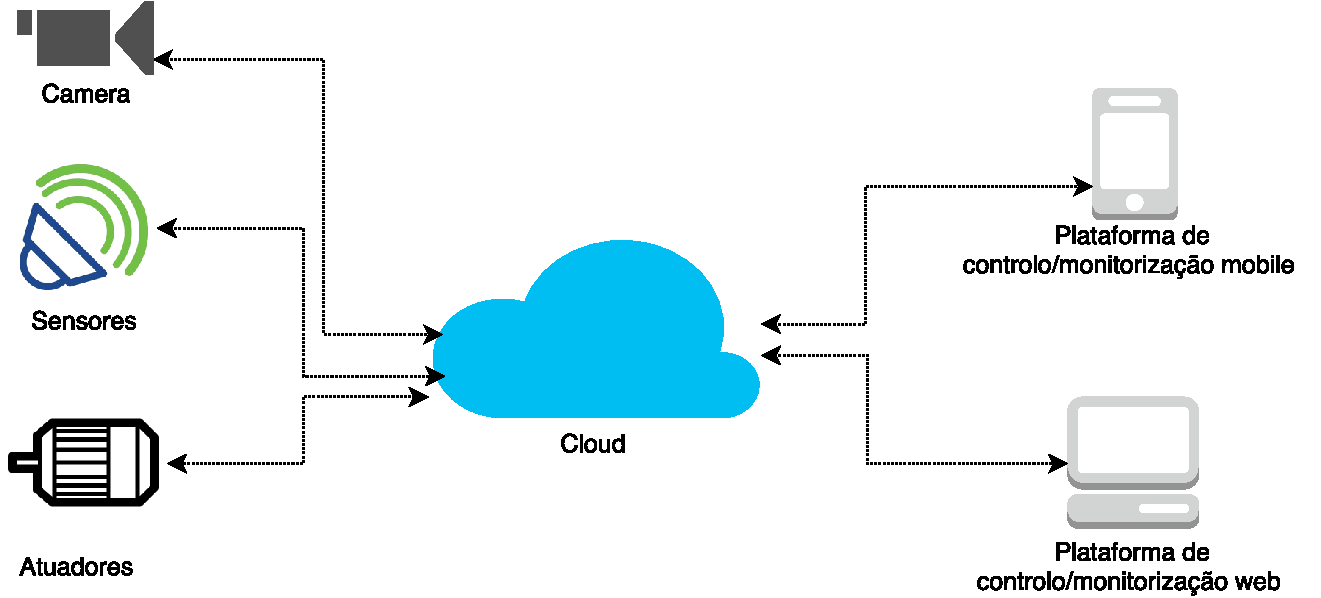
\includegraphics[scale=0.5]{esquemas/global_arquitetura.pdf}
	\caption{Ilustração principais componentes}
	\label{componentesall}
\end{figure}



O esquema da figura \ref{componentesall} ilustra de um modo geral todos os componentes e as diferentes plataformas com que o cliente pode interagir. 


Como vimos no capítulo 3, uma plantação de  Salicórnia carece de um controlo relativamente fino de certos parâmetros ambientais sobretudo da salinidade do terreno onde ela cresce, que depende, das chuvas, da salinidade da água dos canais da ria, entre outros. Nas quintas onde se cultiva salicórnia, a produção faz-se numa espécie de leiras limitadas por pequenos canais de irrigação que podem ser cheios de água salgada proveniente dos esteiros que rodeiam a quinta. Esta operação implica a abertura de válvulas de admissão dessa água, medida do nível da maré nos canais, monitorização da qualidade e salinidade da água exterior.



\begin{figure}[!htb]
	\centering
	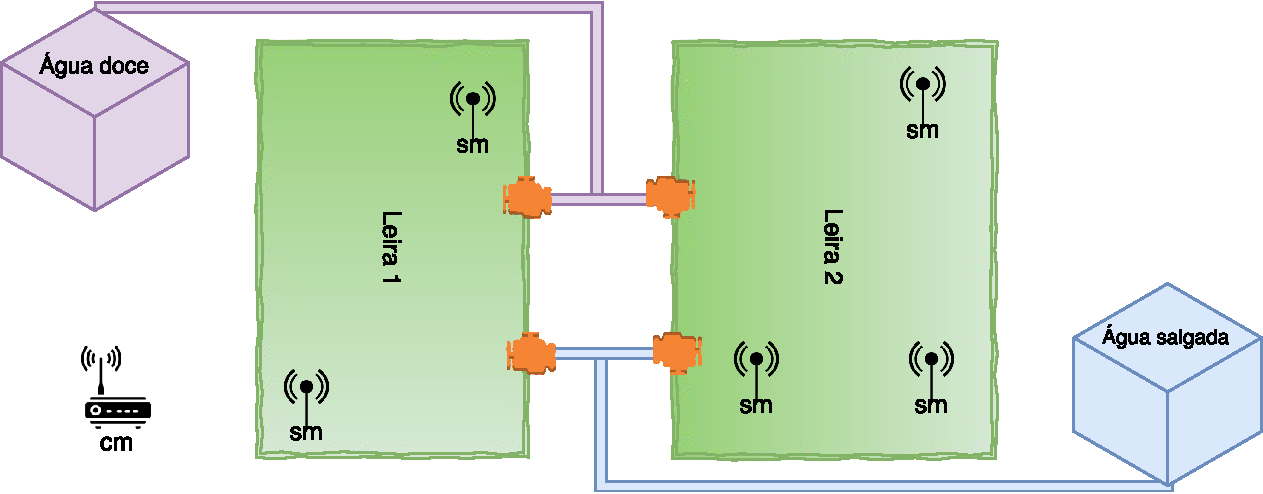
\includegraphics[scale=0.63]{esquemas/leiras-comm-geral.pdf}
	\caption{Ilustração da distribuição dos módulos em duas leiras}
	\label{leira}
\end{figure}


Tal como ilustrado na figura \ref{leira}, pretende-se que sejam colocados módulos com sensores (\acl{SM}) distribuídos estrategicamente por cada leira. Cada um desses módulos, irá comunicar com um módulo central (\acl{CM}) originando uma topologia de rede em estrela.  Por sua vez, cada um destes módulos centrais irá comunicar diretamente com o servidor que permitirá receber todos os dados adquiridos tanto pelos sensores como por atuadores, permitindo que estes sejam guardados numa base de dados especifica. Os atuadores, permitirão despoletar ações que autorizam a ativação ou desativação de bombas e/ou válvulas para transferências de águas de modo a melhorar as condições de cultivo da Salicornia. 
Pretende-se que os módulos centrais tenham acesso à camada protocolar \acs{TCP}/\acs{IP} (Internet) de modo a permitir a utilização da \acs{API} \acs{REST} via \ac{HTTP} desenvolvida para o efeito. 

No que diz respeito às plataformas para interação com o cliente, pretende-se que exista uma \textit{dashboard} e uma aplicação \textit{mobile}. A dashboard disponibilizará  uma interface que apresenta as informações mais importante para o utilizador de forma apelativa, tornando mais fácil a sua interação e respetiva leitura, possibilitando ainda gerir todo o sistema e realizar operações de controlo remoto. Por outro lado, a aplicação \textit{mobile} permitirá apenas a monitorização do cultivo da Salicornia e receção de alertas quando estes ocorram.




\section{Componentes}

No contexto desta dissertação é necessário reter dois conceitos principais, são eles: 

\begin{itemize}
	\item \textbf{\acl{SM}:} consiste num módulo responsável pela aquisição de dados provenientes dos mais diversos tipos de sensores. 
	
	
	\item \textbf{\acl{CM}:} consiste num módulo responsável pela receção dos dados/estados do \acl{SM} e respetivo envio para a \textit{cloud}.  
	
\end{itemize}


O cenário da figura \ref{esquema1} ilustra três \textit{Sensor Modules} que comunicam com um \acl{CM}. Cada um desses \acl{SM} possui um conjunto especifico de sensores, podendo estes ser atuadores ou câmaras. Para a comunicação com o \acl{CM}, cada \acl{SM} possui determinado módulo de comunicação que permita a transferência dos dado adquiridos pelos sensores. Posteriormente, o \acl{CM} possui um determinado protocolo de comunicação (TPC/IP) que permita a utilização da API REST e respetivo envio ou atualização dos dados adquiridos pelo sistema. 



\begin{figure}[h]
	\centering
	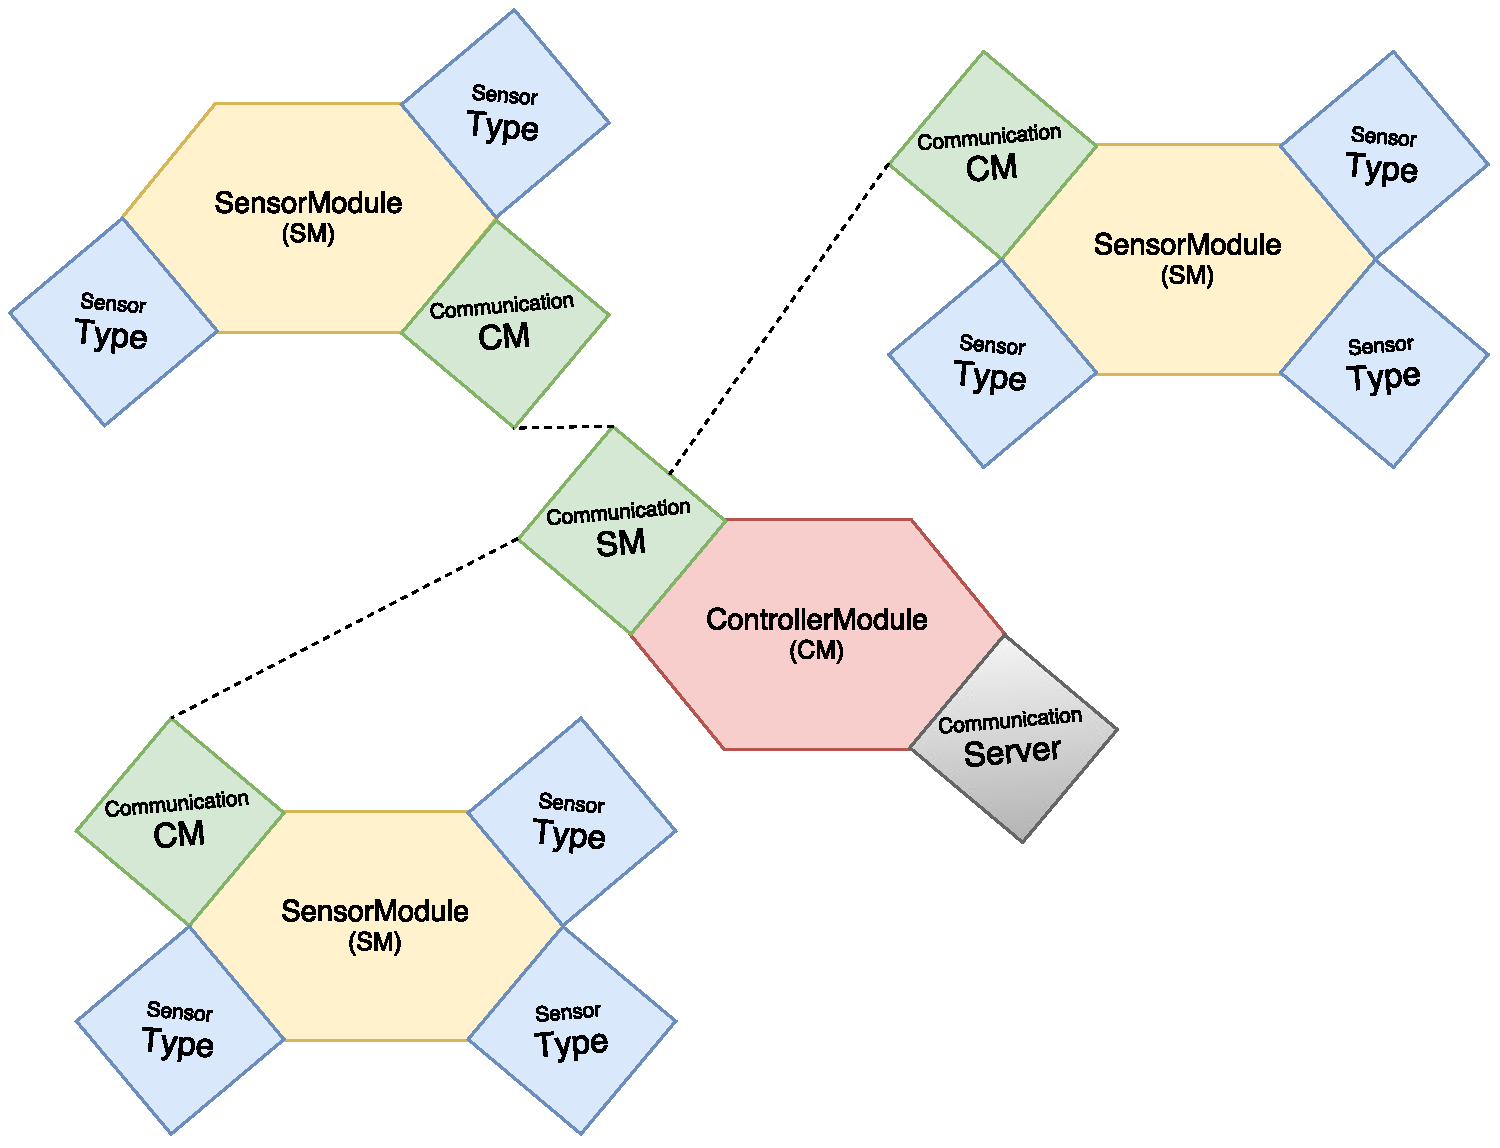
\includegraphics[scale=0.3]{esquemas/general-electronic-modules.pdf}
	\caption{Esquema de componentes e respetiva comunicação entre três \ac{SM} e um \ac{CM}}
	\label{esquema1}
\end{figure}


Seguidamente serão especificados todos os detalhes de cada modulo, uma vez que serão considerados na modelação de todo o sistema. 



\subsection{\acl{SM}}



Um \acl{SM} consiste num micro-controlador responsável pela aquisição de dados provenientes dos mais diversos tipos de sensores, podendo estes ser atuadores ou câmaras. No caso de se tratar de um atuador, isto é, válvulas, bombas, contadores, pás ou cancelas, apenas serão lidos valores binários. Caso se trate de uma câmara, todo o processamento é feito internamente nesta, sendo que o sistema apenas irá receber o IP da mesma. 


Tal como referido anteriormente, cada \acl{SM} terá que utilizar um determinado módulo de comunicação para possibilitar a transferência dos dados adquiridos para o módulo central. Para além disso, pretende-se que o \acl{SM} em condições extremas, possa tomar decisões de atuação, isto é, caso seja lido um valor fora do padrão e que seja necessário a ativação de um atuador, este deverá ser auto suficiente em tomar esta decisão, sem necessidade de intervenção do utilizador. 

Pretende-se que este módulo seja identificado por um determinado nome, possua uma bateria que permita a sua mobilidade, tenha um ou vários módulos de comunicação acoplados que permitam comunicar com um módulo centrar, uma memoria e um módulo \ac{GPS} que permita aceder à sua localização, identificando-o em caso de furto. Para além disso, um \acl{SM} terá que possuir obrigatoriamente um ou vários sensores.








\subsection{\acl{CM}}



Um \acl{CM} consiste num micro-controlador responsável pela receção dos dados prevenientes dos vários \textit{Sensor Modules}. Pretende-se que este módulo envie ou receba informações para os \acl{SM} quando solicitados pelo utilizador. Após a receção dos dados, estes são enviados para um servidor em \textit{cloud} através de uma \ac{API} \ac{REST} criada para o efeito. Sendo que a tecnologia \ac{REST} opera sob o protocolo de comunicação \ac{HTTP}, este componente tem que necessariamente estar ligado à rede Internet via \ac{TCP}/\ac{IP}. 

Pretende-se que este módulo possua alguma capacidade de processamento, uma vez que poderá ter vários \textit{Sensor Modules} a si associados e com necessidade de constante envio e receção de dados.  Para além disso, pretende-se que o \acl{CM} seja identificado por um determinado nome, tenha um  módulo de comunicação que possibilite o envio de dados para um servidor e outros para comunicação com os diferentes \textit{Sensor Modules}. Tal como acontece com os \textit{Sensor Modules}, existe necessidade de acoplado um módulo \ac{GPS} que permita localizar o micro-controlador em caso de robo.
 





\newpage

%\section{Design funcional}






\section{Análise de requisitos}
\label{sect:analise}

Durante o desenvolvimento de \textit{software} pressupõe-se que os seus intervenientes sigam determinadas metodologias para que o seu sistema possa revolucionar a vida de um grupo em especifico ou até mesmo da sociedade. 


O ciclo de vida do desenvolvimento de um software, também conhecido como \ac{SDLC}, é composto genericamente por quatro fases principais: conceção, projeto, criação e a implementação. Antes do \ac{SDLC}, o processo de desenvolvimento do \textit{software} foi tomado como atividade informal sem regras nem padrões formais. Este facto poderá originar vários problemas, tais como o atraso no desenvolvimento, aumento de custos e baixa qualidade do \textit{software} criado. Existem enumerados modelos e visões que propõem alguns padrões e etapas necessárias ao desenvolvimento de um sistema com qualidade.
Na figura \ref{sdlcartic} encontram-se as várias etapas consideradas por \textit{Munish Kaur et al.}\cite{Saini2014}.





\begin{figure}[!htb]
	\centering
	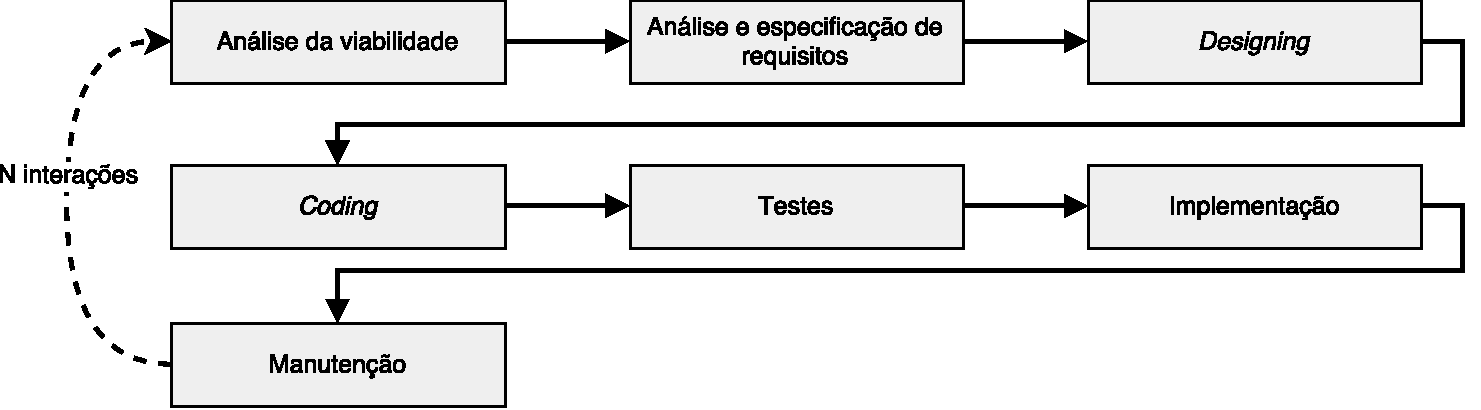
\includegraphics[scale=0.6]{esquemas/desenvolvimentoSW.pdf}
	\caption[Fase de desenvolvimento de um software ]{Fase de desenvolvimento de um software (Adaptado de \cite{Saini2014})}
	\label{sdlcartic}
\end{figure}




\begin{itemize}
	\item \textbf{Análise de viabilidade}: nesta fase são analisados os dados de entrada e saída, processamento necessário, análise de custos e planeamento do projeto. Nesta fase é incluída a viabilidade técnica em termos de \textit{software}, \textit{hardware} e pessoas qualificadas. 
	
	\item \textbf{Análise e especificação de requisitos}: nesta fase são recolhidos e analisados os requisitos necessário para a elaboração do \textit{software}. Pretende-se que no final desta fase sejam conhecidos os vários requisitos do \textit{software} e seja também criado um documento que os especifique. 
	
	\item  \textbf{\textit{Designing}}: consiste na tradução dos requisitos especificado para uma estrutura lógica. Pretende-se que seja elaborado um documento de especificação do \textit{design}. 
	
	
	\item  \textbf{\textit{Coding}}: a programação real é elaborada nesta fase. O documento de \textit{design} é traduzido para o código-fonte numa determinada linguagem de forma a que possa ser executado. 
	
	\item \textbf{Testes}: o código-fonte gerado na fase anterior é testado usando vários cenários de testes. São usadas várias técnicas de teste para avaliar a correção e validação do \textit{software}. 
	
	\item  \textbf{Implementação}: o \textit{software} desenvolvido é implementado para que possa ser disponibilizado ao utilizador para uso real. Pretende-se que o utilizado do sistema possa reportar erros ou problemas quando encontrados. 
	
	\item  \textbf{Manutenção}: o \textit{software} poderá sofrer alterações que possam solucionar problemas que tenham ocorrido. Esta fase é responsável pela pós-implementação e manutenção do \textit{software} para o seu bom funcionamento.
	
\end{itemize}

%http://www.sersc.org/journals/IJSEIA/vol8_no3_2014/38.pdf

Após o entendimento da descrição geral do sistema bem como todos os componentes envolvidos, segue a fase de efectuar o levantamento dos requisitos do sistema, levando-nos a entender o que o cliente deseja ou acredita precisar possibilitando a criação dos processos de negocio necessários ao sistema. Seguidamente serão apresentados os requisitos funcionais e não funcionais deste sistema. 


\subsection{Requisitos funcionais}


Os requisitos funcionais descrevem os critérios que devem ser usados para avaliar as funções especificas ou os comportamentos de um determinado sistema. Os requisitos funcionais que de seguida se apresentam são propostos pelo cliente no contexto deste projeto para as duas plataformas disponíveis: web (\textit{dashboard}) e mobile. \\


\textbf{Aplicação web (\textit{dashboard})}


\begin{itemize}
	\item A interface do sistema deve permitir que o utilizador, seja ele qual for, entre ou faça \textit{login} no sistema. 
	
	\item A interface do sistema deve permitir que o utilizador, seja ele qual for, saia ou faça \textit{logout} no sistema.
	
	\item O \textit{dashboard} deverá permitir que qualquer utilizador possa recuperar a sua chave de acesso ao sistema.

	\item O sistema deve permitir que o utilizador possa adicionar e/ou gerir um ou vários módulos de sensores. 
	
	\item A aplicação web deve permitir visualizar graficamente os dados que cada sensor obtém. 
		
	\item O sistema de permitir visualizar tabularmente (\textit{dataset}) os dados que cada sensor obtém. 
	
	\item Em cada uma das visualizações anteriormente descritas, pretende-se que seja possível efetuar uma filtragem por data.
	
	\item O sistema deverá permitir a exportação dos dados obtidos pelos sensores  em formato \ac{CSV}. 
		
	\item O sistema deve ter a capacidade de gerar alarmes quando algum valor lido pelos sensores esteja fora do previsto. 
	
\end{itemize}


De modo a tornar o sistema genérico e \textit{standalone} foram impostos os seguintes requisitos adicionais: 


\begin{itemize}
	\item O sistema deve permitir que qualquer utilizador se possa registar no sistema, embora tenha que estar obrigatoriamente associado a uma empresa.
	
	\item O utilizador comum só terá acesso à sua área reserva após a validação por parte da empresa.
	
	\item A \textit{dashboard} deverá permitir ao administrador a adição de novas empresas e a gestão de todos os utilizadores. 
	
	
	\item O sistema deve permitir que qualquer utilizador possa adicionar, editar ou remover: 
	\begin{itemize}
		\item Tipos de sensores; 
		
		\item Tipos de comunicação;
		
		\item \acl{CM} com as respetivas especificações e características;
		
		\item Tipo de comunicação a um \acl{CM} que possibilite a sua comunicação como o servidor; 
		
		\item  \textit{Sensor Modules} a um determinado \acl{CM} com as suas respetivas especificações e características; 
		
		\item Um ou vários tipos de comunicação a um \acl{SM} que permita a sua comunicação com um \acl{CM}. 
		
		
		\item Um ou vários sensores a um \acl{SM} em que cada sensor poderá ser de um determinado tipo
	\end{itemize}
	
		
	\item O sistema deverá disponibilizar uma \ac{API} que permita a criação de novas aplicações com base nesta. 
	
	\item Consultar a documentação da \ac{API} de modo interativo. 
	
	\item Gerar e consultar  \textit{token} de autenticação para utilização da \ac{API} 
	
	\item Alterar configurações base de utilizador 
	
\end{itemize}
	


\textbf{Aplicação mobile}



\begin{itemize}
	\item A interface da aplicação mobile deve permitir que o utilizador, seja ele qual for, entre ou faça \textit{login} no sistema. 
	
	\item A interface da aplicação mobile deve permitir que o utilizador, seja ele qual for, saia ou faça \textit{logout} no sistema.
	
	
	\item A aplicação mobile deve permitir visualizar graficamente os dados de cada sensor. 
	
	\item  A aplicação deve permitir receber alarmes quando um determinado valor lido pelo sensor esteja fora do pretendido.
	
	
\end{itemize}



\subsection{Requisitos não funcionais}


Os requisitos não funcionais são todos os requisitos da aplicação relacionados com performance, escalabilidade, segurança, disponibilidade e usabilidade. Estes não são necessariamente pedidos pelo cliente, embora grande parte exista com devido 


\begin{itemize}
	\item O sistema deverá executar em qualquer plataforma, tanto web como mobile. 
	
	
	\item A base de dados deve ser protegida para acesso apenas a utilizadores autorizados. 
		
	
	\item O sistema deverá disponibilizar uma API para que possam ser criados novos produtos com base neste 
	
	\item Deverá ser usada, na medida do possível, tecnologias sem qualquer custo para o cliente (\textit{opensource}). 
	
	\item Pretende-se que o sistema possa ser adaptado a qualquer outro contexto, não sendo especificamente restrito ao contexto da produção da Salicornia.  
		
\end{itemize}


\newpage
\section{Modelação}

Tal como vimos no inicio da secção \ref{sect:analise}, a conceção de uma arquitetura envolve o estudo e respetiva modelação dos componentes que são fundamentais para a realização da mesma, bem como a análise dos casos de uso e respetiva especificação, criação do modelo de dados, diagramas de fluxos, entre outros. Toda esta modelação será descrita neste secção permitindo entender melhor como emparelhar toda a estrutura pretendida. 



\subsection{Entidades envolvidas}

As entidades envolvidas ou atores são os utilizadores do sistema, podendo ser humanos ou entidade máquina, que interagem com o sistema para executar uma determinada ação significativo. No contexto do sistema descrito existem três entidades distintas que são importantes descrever: 

\begin{itemize}
	
	\item \textbf{General user}: este ator poderá registar-se e associando-se a uma determinada empresa existente no sistema. Após a validação por parte da empresa, este utilizador poderá aceder à sua área reservada através da \textit{dashboard} ou da aplicação mobile. 
	
	\item \textbf{Company user}: este utilizador tem a possibilidade de gerir todos os \textit{general users} que se possam associar à sua empresa. Deste modo, este utilizador poderá validar ou remover os \textit{general users} que a si se associam. 
	
	\item \textbf{Administrador}: vulgarmente denominado por Admin. Pretende-se que apenas exista uma único administrador. Este ator tem a possibilidade de adicionar novas empresas ao sistema, isto é, criar novas utilizador com permissões especificas. 
	
\end{itemize}




\subsection{Casos de uso}


Nas figuras \ref{usedash} e \ref{useMobile} encontram-se representados os esquemas dos casos de uso da \textit{dashboard} (denominada por \textit{saliDashboard}) e da aplicação \textit{mobile} (denominada por \textit{saliMobile}), respectivamente.
Seguidamente serão descritos cada um dos casos de uso para as duas plataformas. De notar que todos os casos de uso na aplicação \textit{mobile} também se encontram disponíveis através da \textit{dashboard}. 
\newpage

\begin{figure}[!htb]
	\centering
	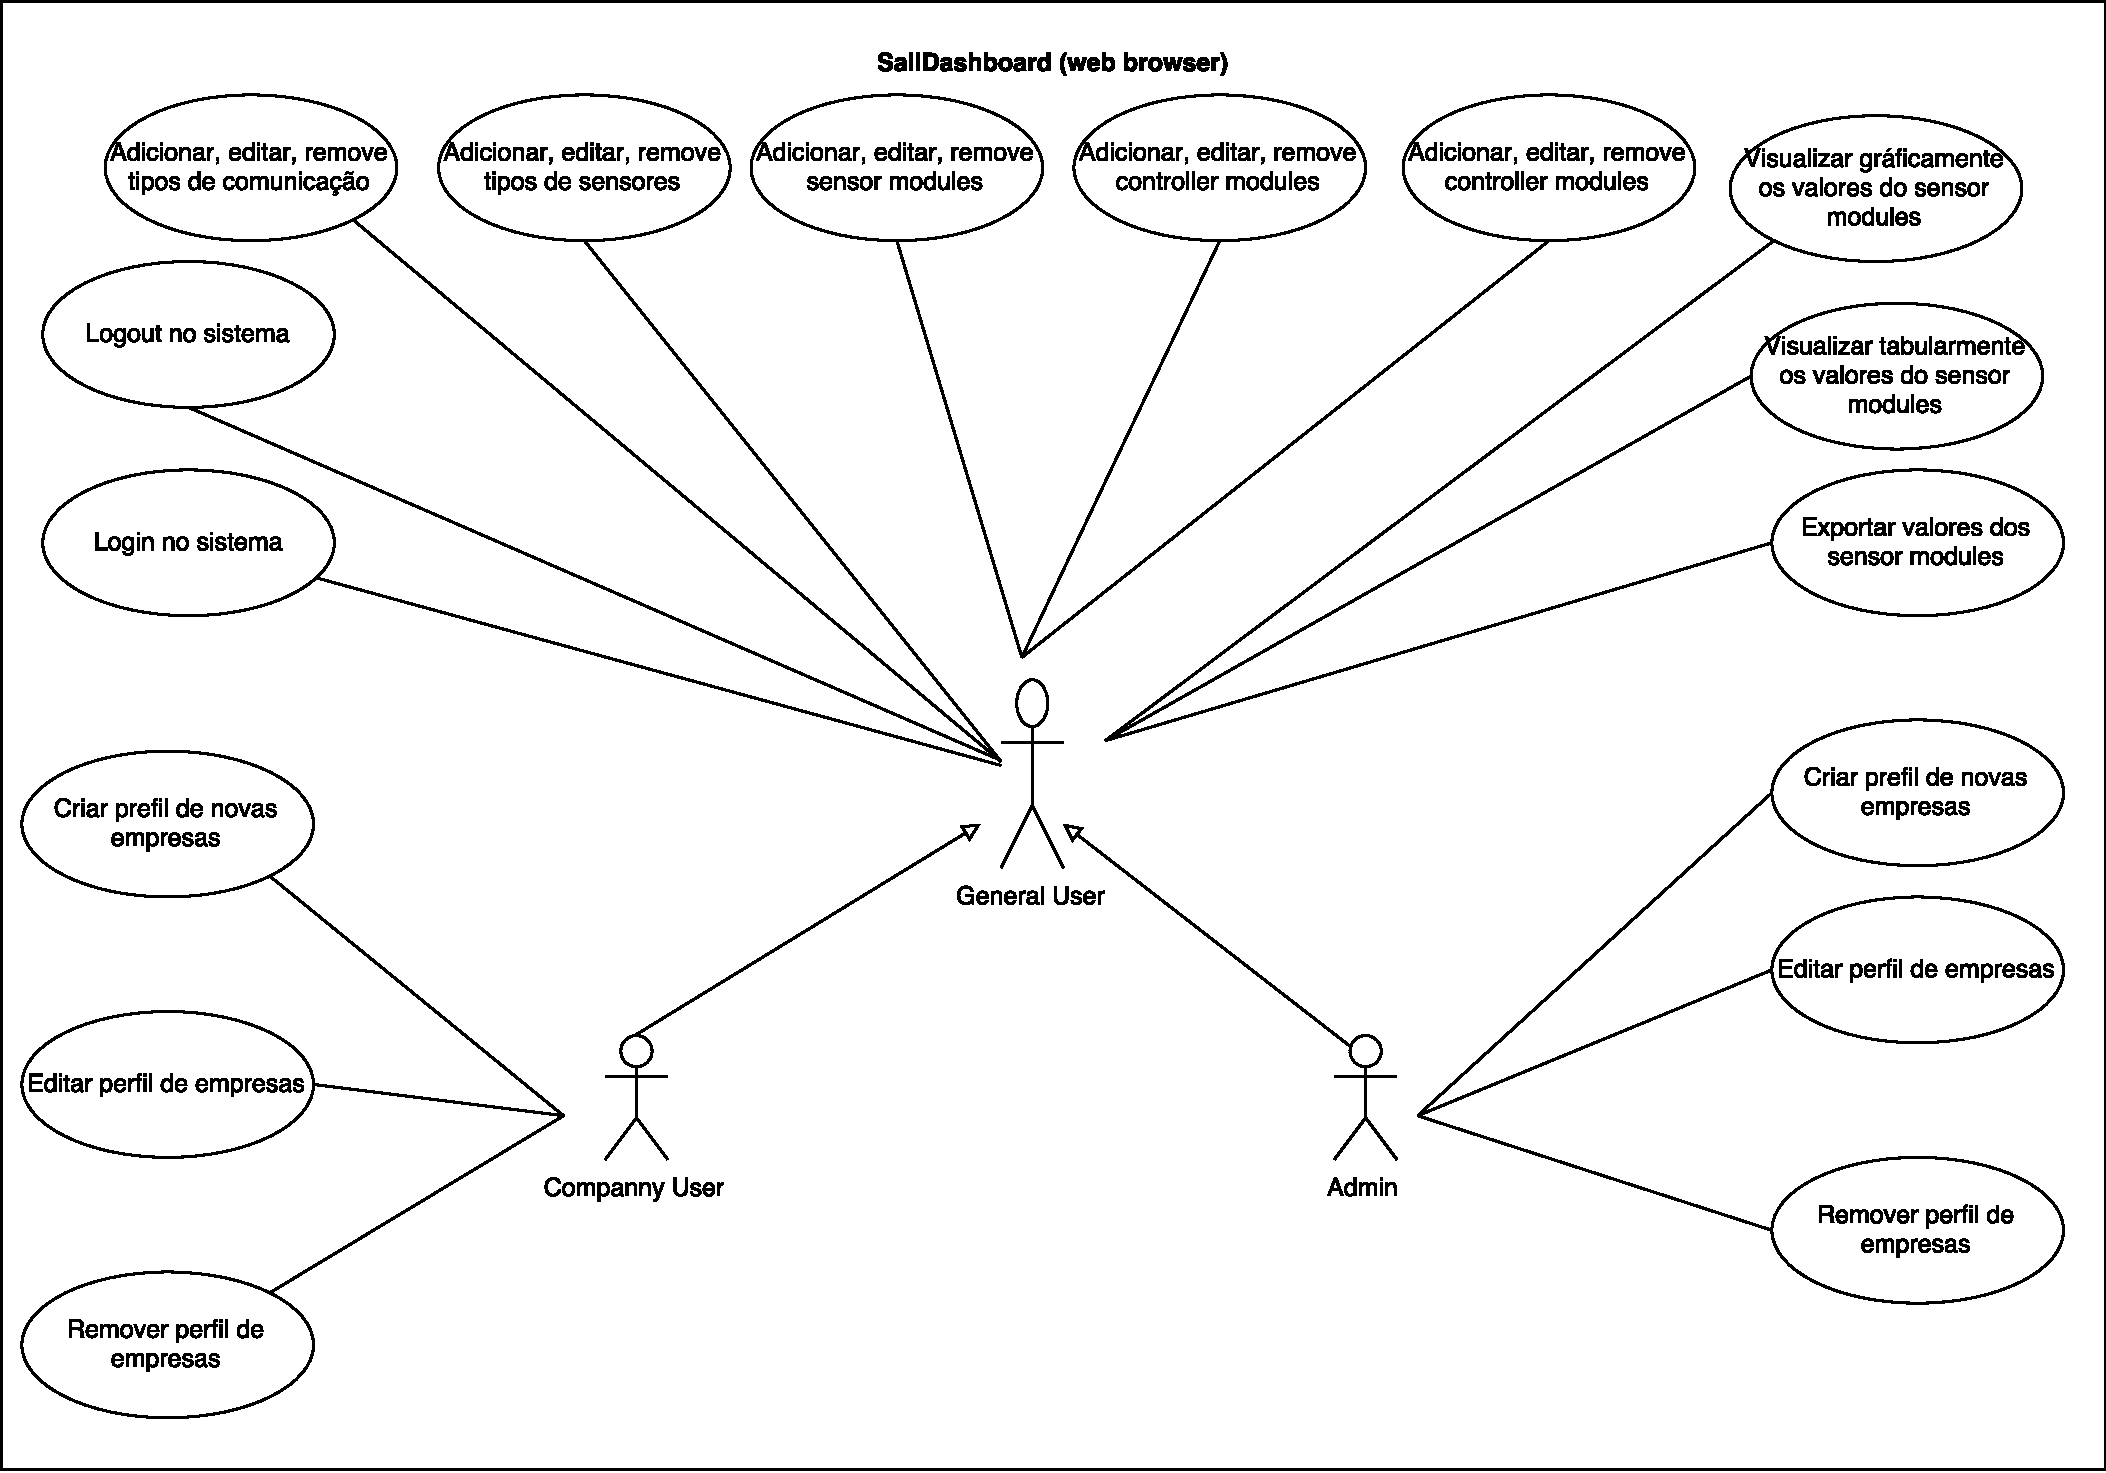
\includegraphics[width=\linewidth]{esquemas/use-case-web.pdf}
	\caption{Casos de uso para a aplicação web (dashboard) }
	\label{usedash}
\end{figure}



\begin{figure}[!htb]
	\centering
	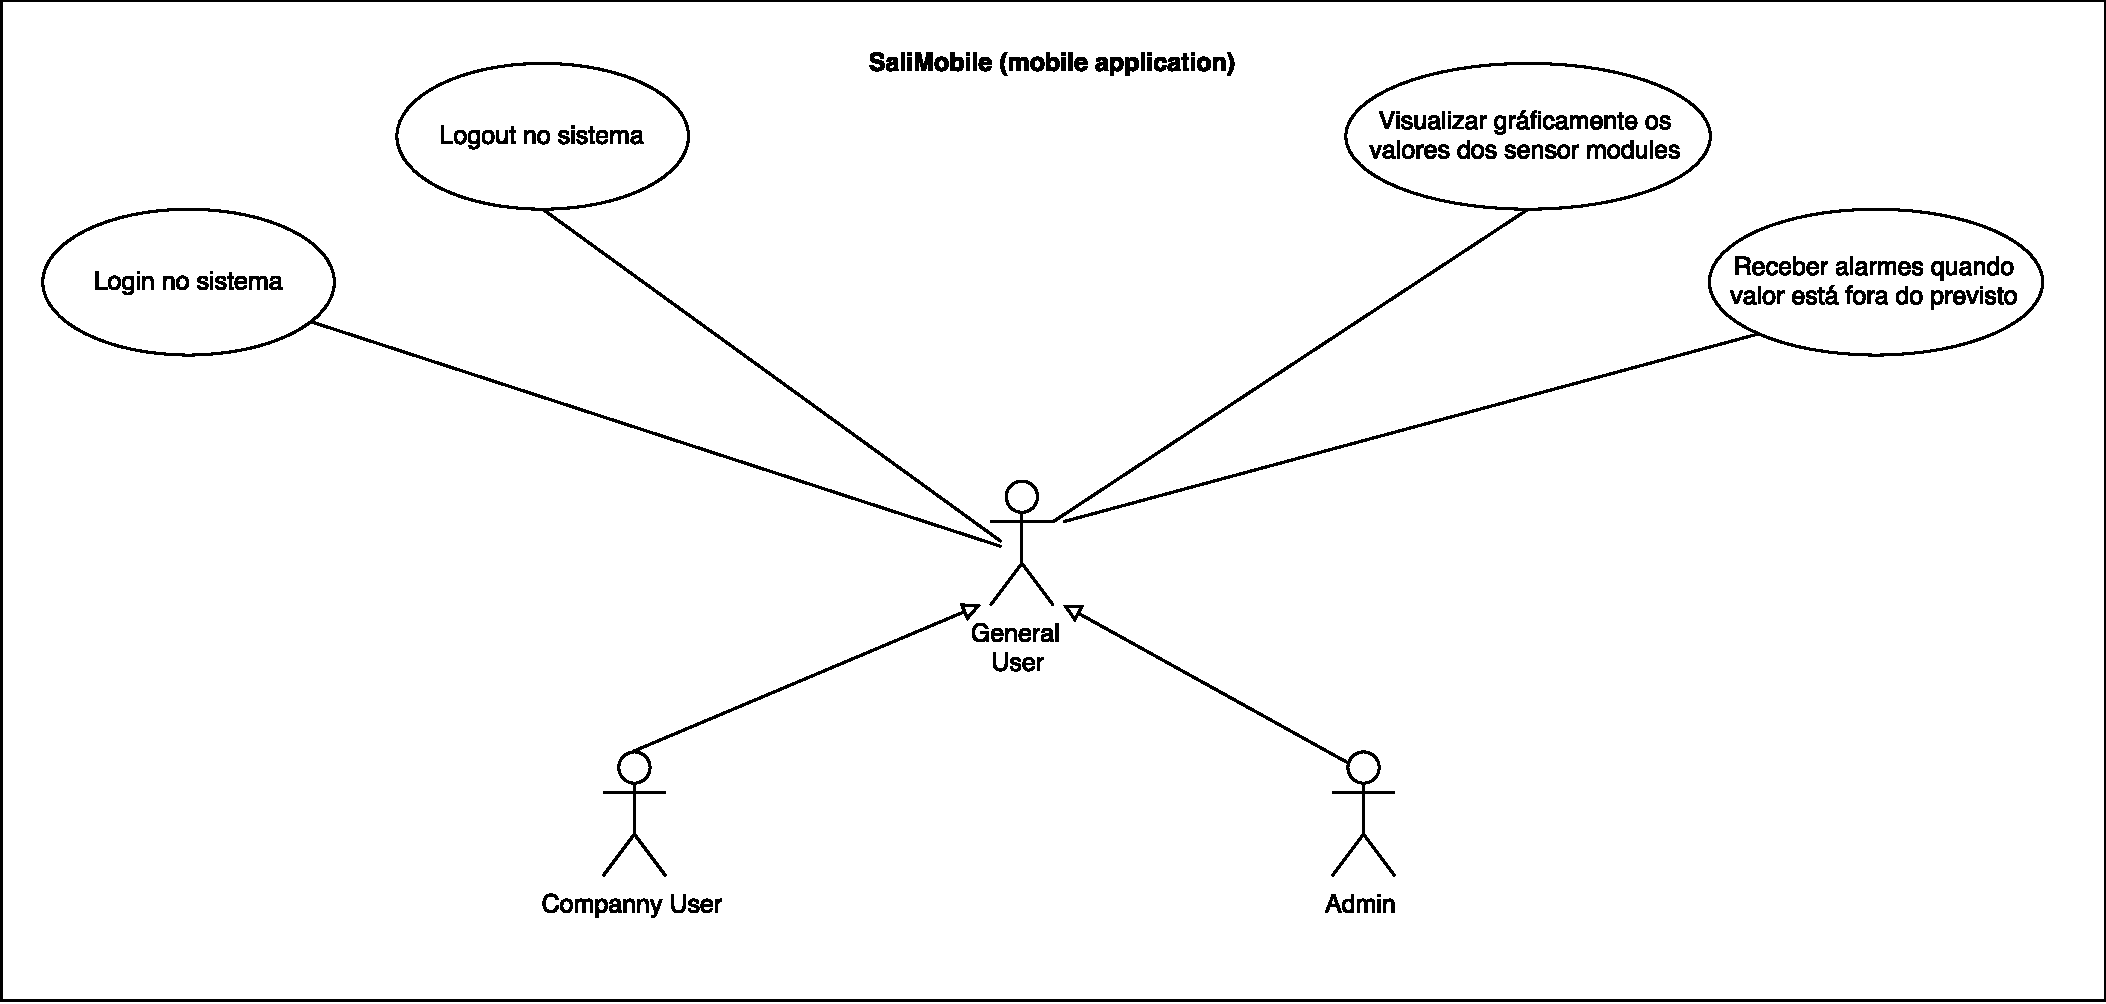
\includegraphics[width=\linewidth]{esquemas/use-case-mobile.pdf}
	\caption{Casos de uso para a aplicação mobile}
	\label{useMobile}
\end{figure}




\newpage
\begin{itemize}
	\item \textbf{Login no sistema}: qualquer utilizador (general user, company user ou admin) poderá aceder ao sistema tendo para isso que possuir uma conta registada e validada no caso do general user. Após a validação das suas credenciais (username e password) o utilizador poderá aceder à pagina inicial da dashboard e a todo o seu conteúdo. Este caso de uso encontra-se disponível para os dois tipos de plataformas. 
	
	
	\item \textbf{Logout no sistema}: qualquer utilizador (general user, company user ou admin) poderá sair da sistema tendo que para isso tenha que estar obrigatoriamente logado no sistema. Após o logout ser-lhe-á apresentado novamente a página de login. Este caso de uso encontra-se disponível para os dois tipos de plataformas. 
	
	
	\item \textbf{Recuperar password}: qualquer utilizador (general user, company user ou admin) poderá recuperar a sua password de acesso ao sistema, para isso, terá que introduzir o seu email e posteriormente ser-lhe-á envia o acesso que possibilita a redefinição da mesma. 
	
	
	
	\item \textbf{Adicionar, editar, remover tipos de comunicação}: qualquer general user ou company user poderá adicionar, editar ou remover os tipos de comunicação existentes no sistema. Ao  adicionar, o utilizador terá que introduzir um nome, um caminho relevante para o tipo de comunicação e selecionar um icon ilustrativo. No caso da remoção, esta ação apenas é possível caso o tipo de comunicação não se encontre em utilização por nenhum \ac{CM} ou \ac{SM}.  
	
	\item \textbf{Adicionar, editar, remover tipos de sensores}: qualquer general user ou company user poderá adicionar, editar ou remover os tipos de sensores existentes no sistema. Ao  adicionar, o utilizador terá que introduzir um nome que o identifique, uma fonte de dados ou a escala dos dados  e um icon que identifique o sensor. Para além disso, o utilizador terá que escolher uma cor que identifique o tipo de sensor na dashboard. No caso da remoção, esta ação apenas é possível caso o tipo de sensor não se encontre em utilização por nenhum \ac{SM}.   
	 
	
	\item \textbf{Adicionar, editar, remover um controller module}: qualquer \textit{general user} ou \textit{company user} poderá adicionar, editar ou remover um controller module existente no sistema. Neste caso, pressupõe-se que o utilizador possua um micro-controlador com as seguintes características que podem ser adicionadas: determinado nome que o identifique, valor da memória RAM em MB, estado inicial (ativo ou desativo) e um modulo de comunicação que permita comunicar com o servidor web. Estas características são possíveis de alteração. Pretende-se que o controller module possa ser removido tendo \ac{SM} a sí associado, sendo estes também removidos dos sistema. 


	\item \textbf{Adicionar, editar, remover um sensor modules}: qualquer \textit{general user} ou \textit{company user} poderá adicionar, editar ou remover um sensor module existente no sistema. Pressupõe-se o utilizador possui um determinado micro-controlador com um ou mais sensores. Para adicionar o \ac{SM} à plataforma o utilizador terá que atribuir um nome que o identifique, definir qual o seu estado inicial (ativo ou desativo), escolher que tipos de comunicação possam estar presentes e definir o intervalo de tempo para o qual pretende receber os dados lidos pelos sensores. Para além disso, permite associar ao \ac{SM} os sensores presentes e definir o valor máximo e minimos para o qual são gerados alarmes e respectivas mensagens informativas. Todos os dados são possíveis de edição.  
	

	
	\item \textbf{Receber notificações (gerar alarmes)}: sempre que um valor lido por um determinado sensor sai fora do limite imposto (valor máximo e valor mínimo) é gerado um alarme para o utilizador de modo a que este possa intervir. Este caso de uso encontra-se disponível para os dois tipos de plataformas. 
	
	
	\item \textbf{Visualizar gráficamente os dados lidos pelos sensores}: 
	
	
	Este caso de uso encontra-se disponível para os dois tipos de plataformas. 
	
	
	\item Visualizar tabularmente os dados lidos pelos sensor
	
	\item \textbf{Exportar dados lidos por um sensor module}: qualquer \textit{general user} ou \textit{company user} poderá exportar os dados lido pelos sensores para um ficheiro do tipo \ac{CSV} para uma data especificada.
	
	\item \textbf{Visualizar a localização dos módulos (SM/CM)}: qualquer \textit{general user} ou \textit{company user} ao aceder à dashboard ser-lhe-à apresentado um mapa para cada \ac{CM} com a sua localização e dos seus respetivos \ac{SM}. 
	
	
	\item \textbf{Consultar a documentação da API}: qualquer \textit{general user} ou \textit{company user} poderá aceder à dashboard para consultar a documentação da API existente. 
		
	\item \textbf{Consultar token de autenticação}: qualquer \textit{general user} ou \textit{company user} poderá aceder ao token de autenticação para utilização da API. 
	

	
	\item \textbf{Validar general user}: qualquer company user tem a possibilidade de validar os general users que a si se associam. Sempre um novo general user é registado no sistema o comapny user é notificado via email. Posteriormente, caso o general user seja validado este também receberá um email de confirmação.  
	
	\item \textbf{Remove general user}: qualquer company user tem a possibilidade de remove os general users que a si estão associados. 
	
	
	\item \textbf{Remover sensor modules e controller modules }: o admin do sistema tem a possibilidade de remover os sensores modules e/ou controller modules existentes no sistema. 
	
	
	\item \textbf{Visualizar todos os sensor modules e controller modules}: o admim do sistema tem a possibilidade de visualizar todos os sensores modules e controller modules existentes no sistema de modo a alertar os clientes em caso de anomalias. 
	
	
	\item \textbf{Criar um novo company user}: o admim tem a possibilidade de adicionar novos company user ao sistema, sendo para isso necessário 
	
	\item \textbf{Remover um company user}: o admim tem a possibilidade de remover qualquer company user registado no sistema.
	
	
\end{itemize}










\newpage
\subsection{Modelo de dados}

Depois da análise de requisitos desenhou-se um modelo de dados que permitisse modelar todo o sistema descrito, obtendo-se assim o seguinte esquema relacional apresentado na figura \ref{esquemarelacional}.





\begin{figure}[!htb]
	\centering
	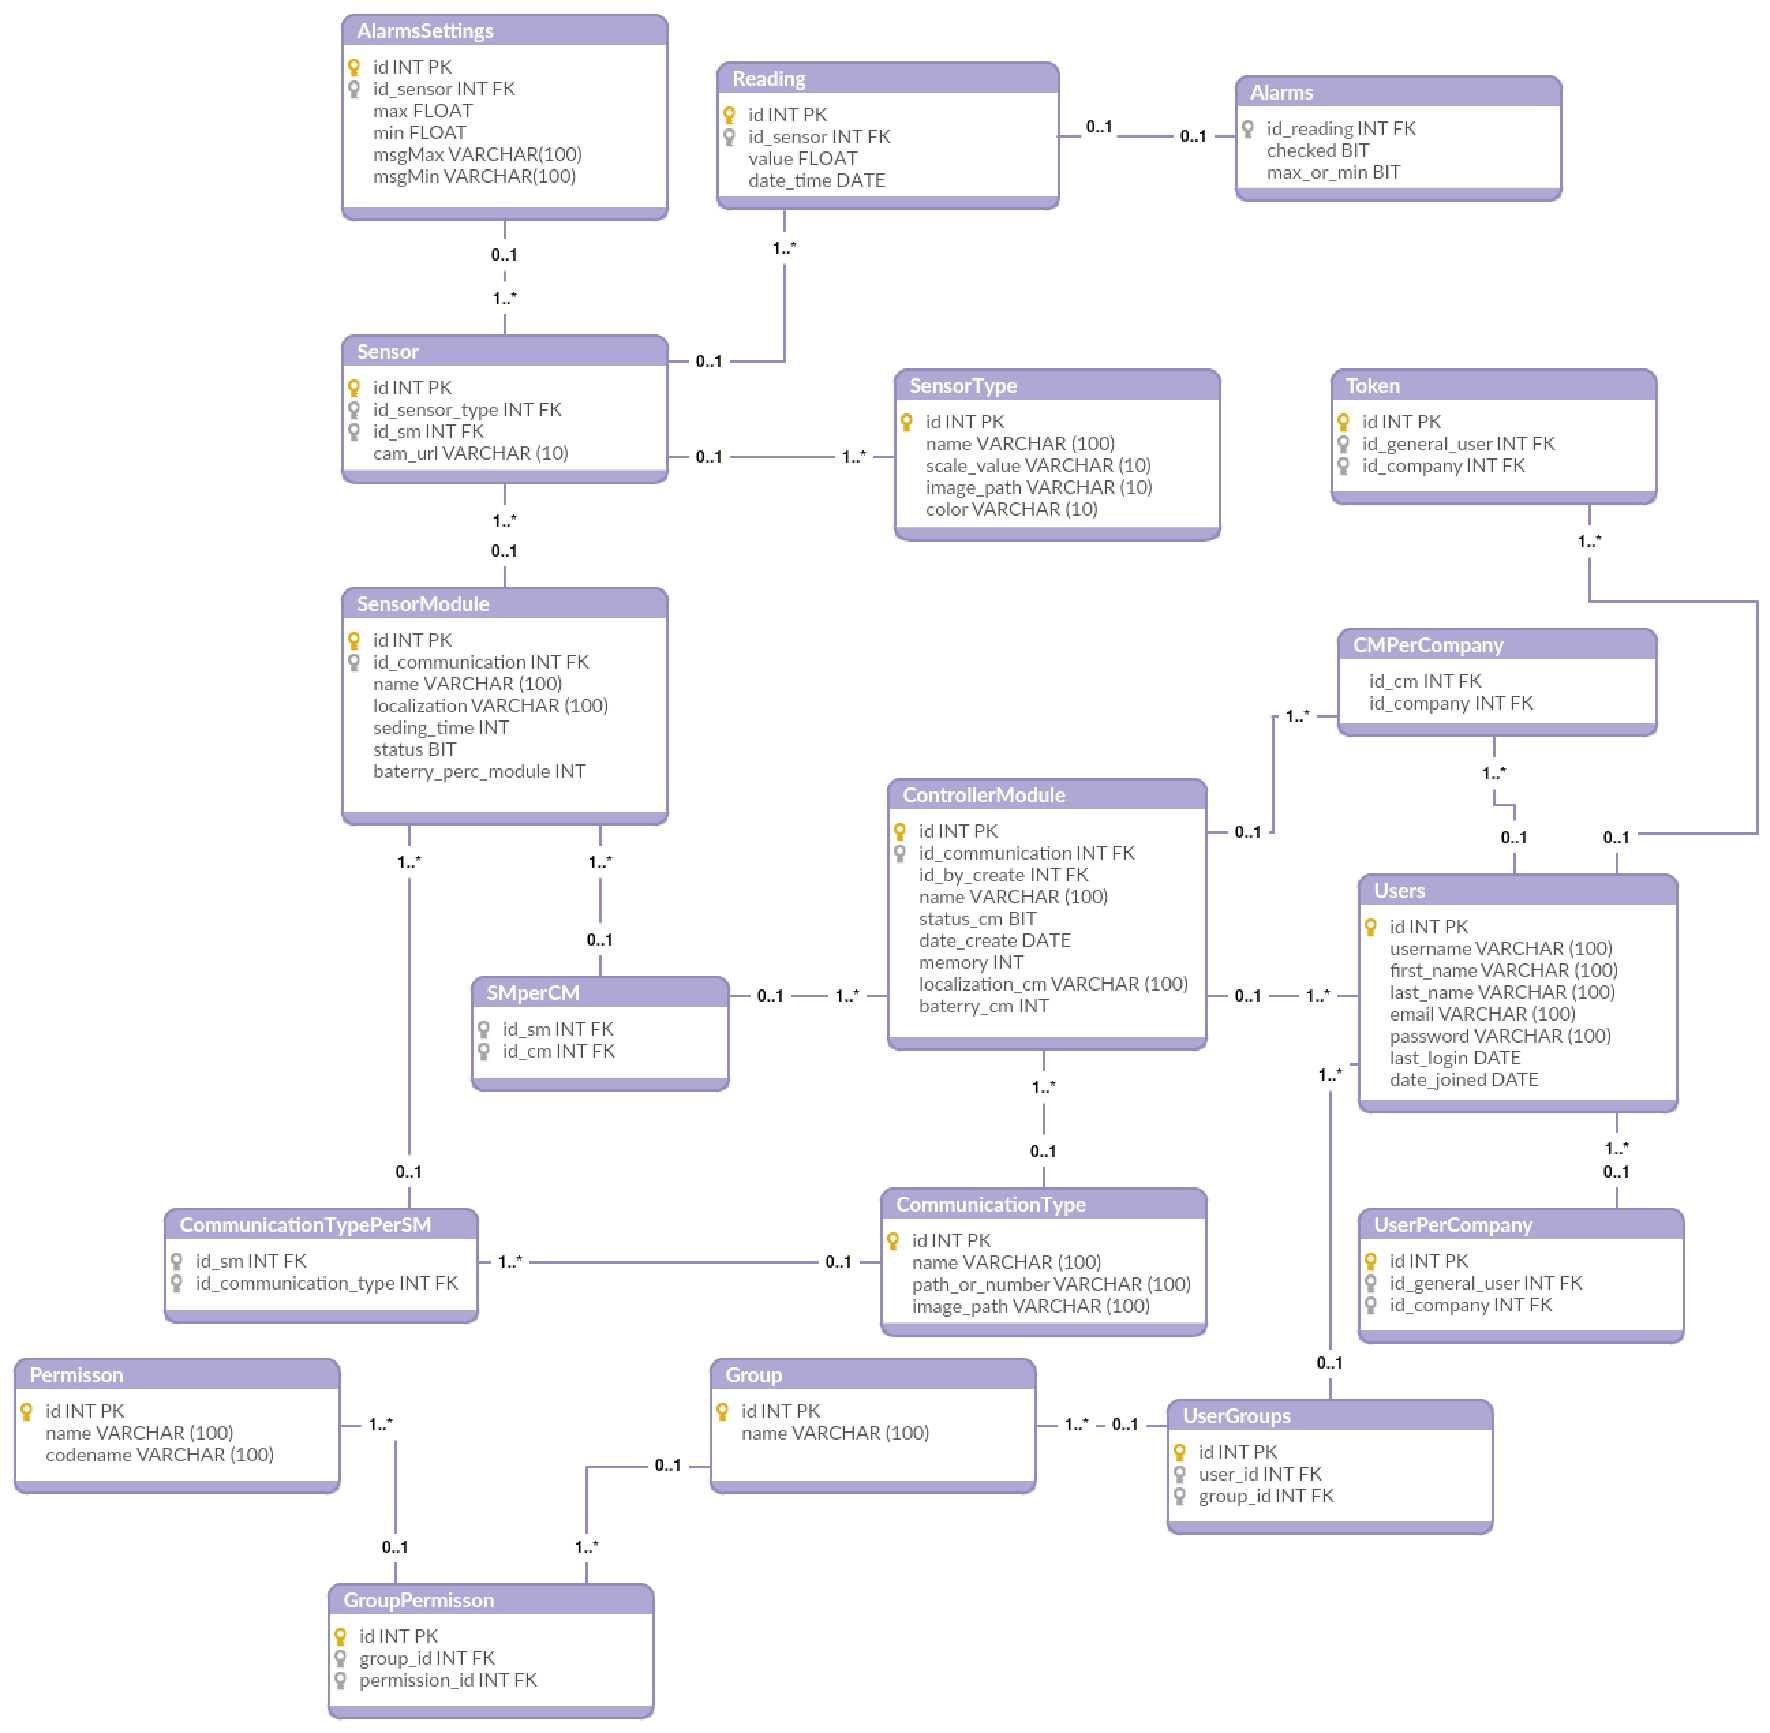
\includegraphics[width=\linewidth]{esquemas/database_tese.pdf}
	\caption{Esquema relacional da estrutura da base de dados}
	\label{esquemarelacional}
\end{figure}


Nas tabelas \ref{tabeladb1} e \ref{tabeladb2} são descritos cada uma das entidades de dados existente neste sistema, evidenciando as chaves primária e estrangeiras de cada uma. 



\newpage
\begin{landscape}
	
\begin{table}[]
	\centering

	
	\begin{tabular}{|
			>{\columncolor[HTML]{EFEFEF}}l |l|l|l|}
		\hline
		\textbf{Nome da tabela} & \cellcolor[HTML]{EFEFEF}\textbf{Chave primária (\acs{PK})} & \cellcolor[HTML]{EFEFEF}\textbf{Chave estrangeira (\acs{FK})} & \cellcolor[HTML]{EFEFEF}\textbf{Descrição} \\ \hline
		\textbf{User} & id (auto-incrementado) & N/A & \begin{tabular}[c]{@{}l@{}}Identifica cada um dos \\ utilizadores inseridos no sistema\end{tabular} \\ \hline
		\textbf{Token} & \begin{tabular}[c]{@{}l@{}}authtoken\_token\_pkey\\ (character varying(40))\end{tabular} & user\_id & \begin{tabular}[c]{@{}l@{}}Possui o token de autenticação \\ do utilizador para a API\end{tabular} \\ \hline
		\textbf{Group} & id (auto-incrementado) & N/A & \begin{tabular}[c]{@{}l@{}}Possui todos os grupos \\ existentes: general user,\\ company user e admin\end{tabular} \\ \hline
		\textbf{UserGroups} & id (auto-incrementado) & user\_id group\_id & \begin{tabular}[c]{@{}l@{}}Permite associar um \\ utilizador a um\\  determinado grupo\end{tabular} \\ \hline
		\textbf{Permisson} & id (auto-incrementado) & N/A & \begin{tabular}[c]{@{}l@{}}Possui todas as permissões \\ existentes (escrita, leitura,\\  delete...)\end{tabular} \\ \hline
		\textbf{GroupPermisson} & id (auto-incrementado) & group\_id permission\_id & \begin{tabular}[c]{@{}l@{}}Associa a cada groupo \\ determinadas permissões\end{tabular} \\ \hline
		\textbf{UserPerCompany} & id (auto-incrementado) & company\_id general\_user\_id & \begin{tabular}[c]{@{}l@{}}Associa cada general user\\  a um company user\end{tabular} \\ \hline
		\textbf{CommunicationType} & id (auto-incrementado) & N/A & \begin{tabular}[c]{@{}l@{}}Identifica cada um dos tipos \\ de comunicação inseridos \\ no sistema\end{tabular} \\ \hline
		\textbf{ControllerModule} & id (auto-incrementado) & N/A & \begin{tabular}[c]{@{}l@{}}Identifica cada um dos \\ controller module \\ inseridos no sistema\end{tabular} \\ \hline
	\end{tabular}
	\caption{Especificação das tabelas existentes no sistema }
	\label{tabeladb1}
\end{table}


\newpage




\begin{table}[]
	\centering

	
	\begin{tabular}{|
			>{\columncolor[HTML]{EFEFEF}}l |l|l|l|}
		\hline
		\multicolumn{1}{|c|}{\cellcolor[HTML]{EFEFEF}\textbf{Nome da tabela}} & \multicolumn{1}{c|}{\cellcolor[HTML]{EFEFEF}\textbf{Chave primária (PK)}} & \multicolumn{1}{c|}{\cellcolor[HTML]{EFEFEF}\textbf{Chave estrangeira (FK)}} & \multicolumn{1}{c|}{\cellcolor[HTML]{EFEFEF}\textbf{Descrição}} \\ \hline
		\textbf{CMPerCompany} & id (auto-incrementado) & \begin{tabular}[c]{@{}l@{}}cm\_id\\ company\_id\end{tabular} & \begin{tabular}[c]{@{}l@{}}Associa todos os controller module\\  a um determinado company user\end{tabular} \\ \hline
		\textbf{SensorModule} & id (auto-incrementado) & N/A & \begin{tabular}[c]{@{}l@{}}Identifica cada um dos sensor \\ module inseridos no sistema\end{tabular} \\ \hline
		\textbf{SMperCM} & id (auto-incrementado) & \begin{tabular}[c]{@{}l@{}}cm\_id\\ sm\_id\end{tabular} & \begin{tabular}[c]{@{}l@{}}Associa os sensor modules a \\ um determinado controller module\end{tabular} \\ \hline
		\textbf{CommunicationTypePerSM} & id (auto-incrementado) & \begin{tabular}[c]{@{}l@{}}communication\_type\_id\\ \\ sm\_id\end{tabular} & \begin{tabular}[c]{@{}l@{}}Permite associar a um sensor \\ module um ou várias tipos \\ de comunicação\end{tabular} \\ \hline
		\textbf{SensorType} & id (auto-incrementado) & N/A & \begin{tabular}[c]{@{}l@{}}Identifica cada um dos tipos \\ de sensores inseridos no sistema\end{tabular} \\ \hline
		\textbf{Sensor} & id (auto-incrementado) & \begin{tabular}[c]{@{}l@{}}sensor\_type\_id\\ sm\_id\end{tabular} & \begin{tabular}[c]{@{}l@{}}Permite identificar um \\ determinado sensor\end{tabular} \\ \hline
		\textbf{AlarmsSettings} & id (auto-incrementado) & sensor\_id & \begin{tabular}[c]{@{}l@{}}Permite guardar as configurações \\ para um determinado sensor\\ (max,min…)\end{tabular} \\ \hline
		\textbf{Reading} & id (auto-incrementado) & sensor\_id & \begin{tabular}[c]{@{}l@{}}Permite guardar as leituras de \\ um determinado sensor\end{tabular} \\ \hline
		\textbf{Alarms} & id (auto-incrementado) & reading\_id & \begin{tabular}[c]{@{}l@{}}Armazena os alarmes \\ que são gerados\end{tabular} \\ \hline
	\end{tabular}
	\caption{Especificação das tabelas existentes no sistema (continuação) }
	\label{tabeladb2}
\end{table}

\end{landscape}



\newpage
\section{Arquitetura lógica}

Nesta secção é apresentada uma arquitetura lógica do sistema, indicando as camadas que contém, especificando quais as relações de dependência que estas possuem entre si. Seguidamente, é explicado como implementar esta lógica com os respetivos componentes físicos. 


Normalmente este tipo de arquitetura é composto por três camadas com intenções diferentes: camada de apresentação, camada de lógica de negócio e camada de acesso a dados. Pretende-se que com a descrição desta arquitetura seja facilitada a manutenção, a portabilidade e a
escalabilidade, fatores importantes quando queremos partilhar funcionalidades e informação entre aplicações de diferentes tipos.




\begin{figure}[!htb]
	\centering
	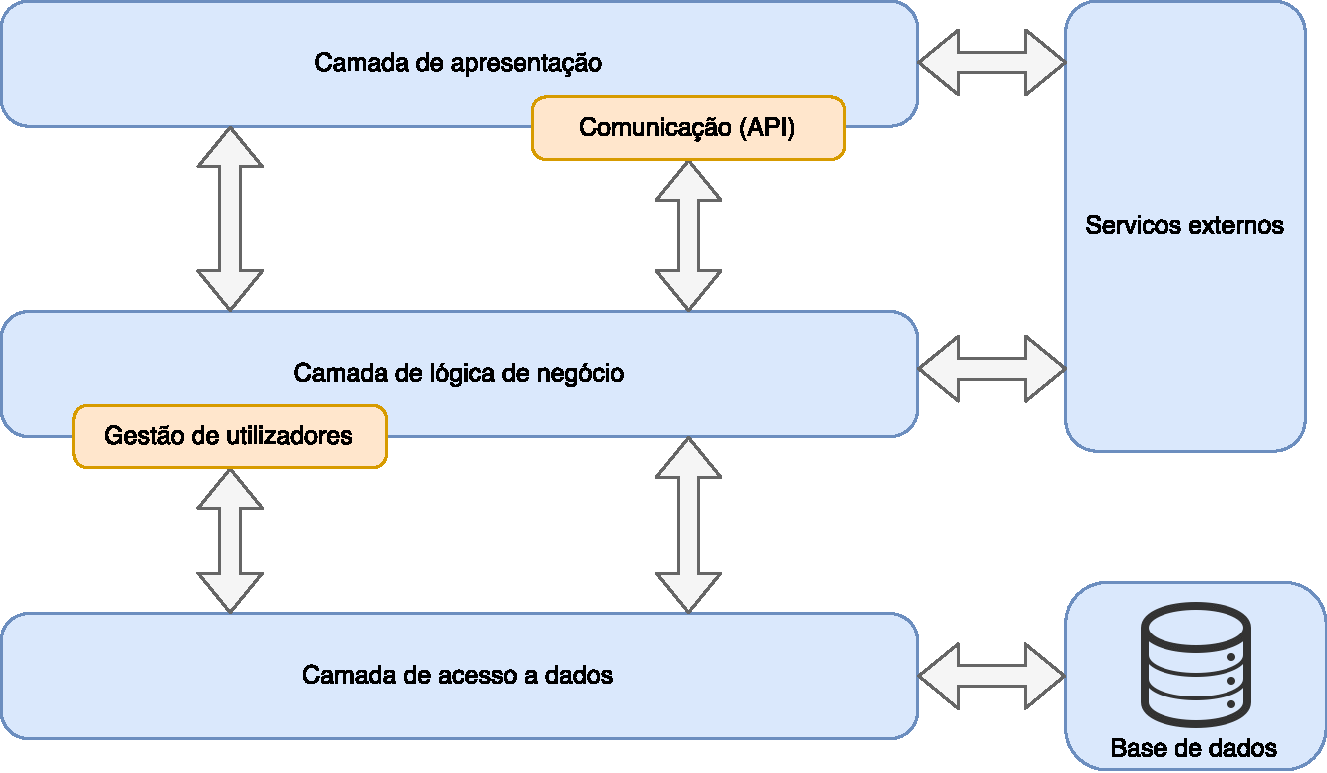
\includegraphics[scale = 0.6]{esquemas/arquitetura-logica.pdf}
	\caption{Arquitetura lógica}
	\label{logicaarqu}
\end{figure}



A camada de apresentação é responsável pela comunicação entre os utilizadores e a aplicação, sendo ela \textit{web} ou \textit{mobile}, exibindo informações aos utilizadores, abrangendo uma interface que permite solicitações ao sistema. Esta camada tem uma relação de dependência com a camada de lógica de negócio e tira partido do acesso a serviços de informação externos, que fornecem diversas funcionalidades. A interface do utilizador foi desenvolvida em  \ac{HTML} e \acs{CSS}, fazendo uso de jQuery e Javascript.





A camada de lógica de negócio diz respeito à camada onde é realizado todo o processamento dos dados adquiridos pelos sensores ou introduzidos pelos utilizadores do sistema através da camada de apresentação.  Tal como apresentado na figura \ref{logicaarqu}, existem quatro sub-camadas principais, que enfatizam os principiais conceitos existentes nesta camada, a seguir descritos.  


\begin{itemize}
	\item \textbf{Gestão de utilizadores}: todas as operações realizadas por cada utilizador devem ser medidas pelas permissões que estes possuem. Nesta camada é verificado se um determinado utilizador viola ou não essas permissões. 
	
	\item \textbf{Geração de alarmes}: todos os alarmes são gerados conforme a verificação automática realizada a cada valor que chega ao sistema. 
	\item \textbf{Cálculos estatísticos}: este componente da camada de lógica de negócio ganha especial relevância na altura em que se pretende determinar os valores médios, máximos e minimos de um conjunto de medições para um determinado intervalo de tempo. 
	\item \textbf{Comunicação via \ac{API}}: este componente é fundamental para que se possa aceder, atualizar ou adicionar dados ao sistema de um modo simples.
\end{itemize}



Relativamente à camada de acesso a dados, deverão estar presentes as funcionalidades de criação, edição, remoção ou simples de visualização dos dados, sendo responsável pelas operações de persistência e consulta de dados solicitadas pela camada de lógica de negócio.


\section{Arquitetura física}


Enquanto que a arquitetura lógica se concentra nos diferentes níveis de abstração do sistema a arquitetura física foca-se na estrutura de alto nível.  
Seguidamente são apresentados todos os componentes físicos, tanto  a nível de \textit{software} com de \textit{hardware}, que são fundamentais para ter um maior perceção do real funcionamento de todo o sistema. 
A figura \ref{fisicablocos} representa genericamente os blocos principais do sistema proposto que seguidamente serão descritos. 


\begin{figure}[h]
	\centering
	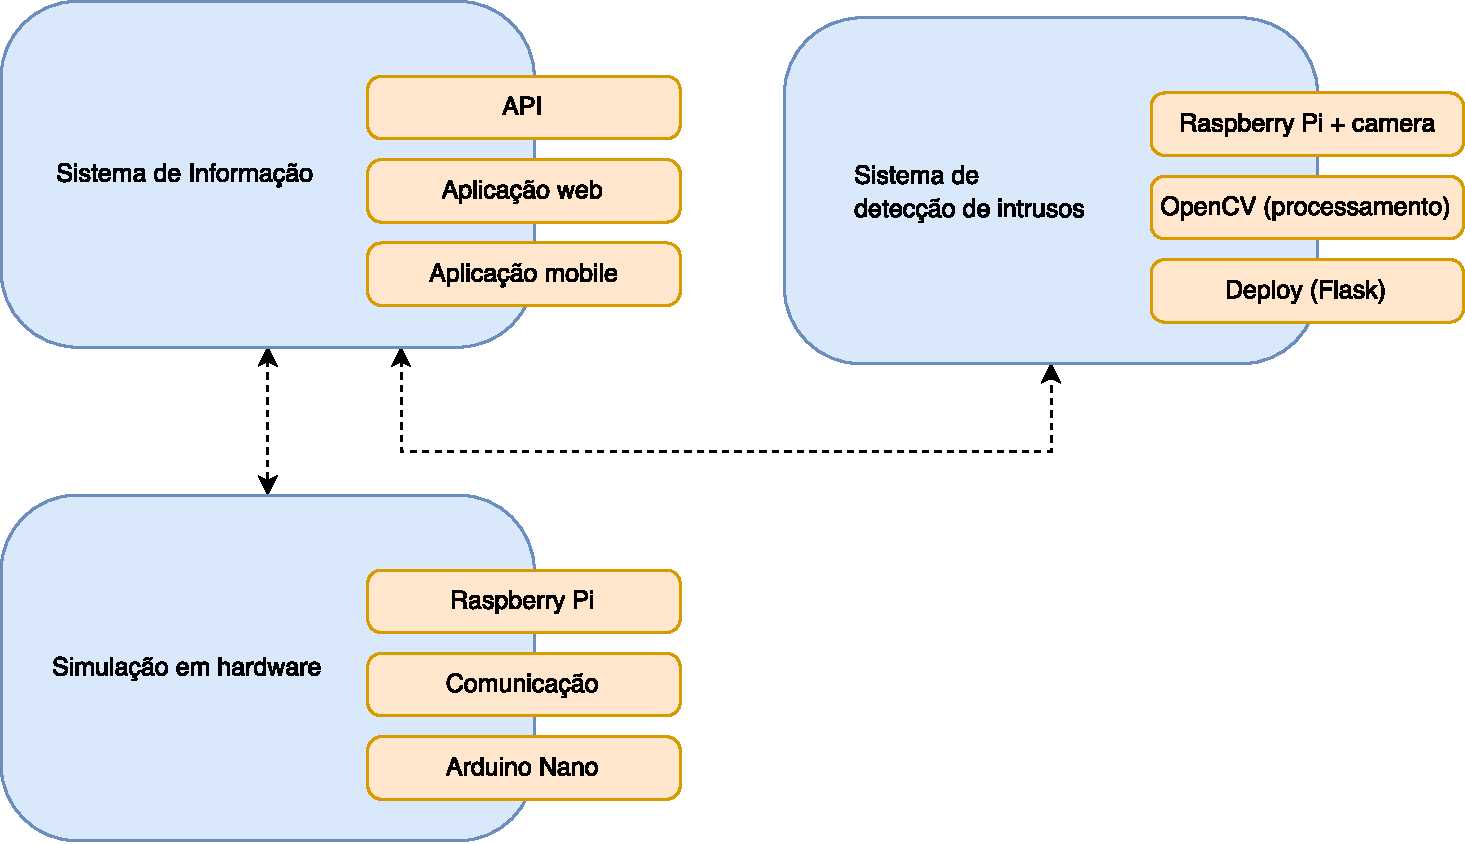
\includegraphics[scale=0.41]{esquemas/esquema-blocos.pdf}
	\caption{Arquitetura física (blocos)}
	\label{fisicablocos}
\end{figure}


  
\subsection{Sistema de informação}


Segundo \textit{Laudon et al.}\cite{Laudon1998} um sistema de informação define-se como sendo uma inter-relação de múltiplos componente podendo estes ser equipamentos, telecomunicações, \textit{software}, bases de dados e outras tecnologias de transformação de informação. Todos estes componentes permitem a recolha, processamento, armazenamento e distribuição de informação que possibilita a tomada de decisões e controlo para uma determinada organização, ou até mesmo para a sociedade, de modo a torná-la mais acessível e útil.

Dada a elevada complexidade de um sistema de informação, é possivel identificar algumas funcionalidade comuns aos diversos sistema existentes, são eles\cite{Turban1996}: 

\begin{itemize}
	\item \textbf{Recolha de dados}: sequência de tarefas que permitem a adição de novos dados ao sistema.
	
	\item \textbf{Organização e armazenamento de dados}: é imprescindível uma boa organização na estrutura de dados possibilitando uma fácil e rápida localização.
	\item \textbf{Processamento de dados}: qualquer funcinalidade que permita a produção de resultados mais úteis do que os dados em bruto. 
	 
	\item \textbf{Distribuição de informação}: após o processamento de dados é fundamental a distribuição destes a quem precise deles.
	
	\item \textbf{Utilização da informação}: por si só, a informação não tem qualquer valor, a sua utilização em contexto adequado permite a extração de determinadas conclusões para que possam ser tomadas decisões.
	
\end{itemize}



A figura \ref{arquiteturasi} ilustra a arquitetura do sistema de informação incluindo especificamente a aplicação web (\textit{dashboard}), base de dados, \acs{API}   e respetiva implementação do sistema. 


\begin{figure}[h]
	\centering
	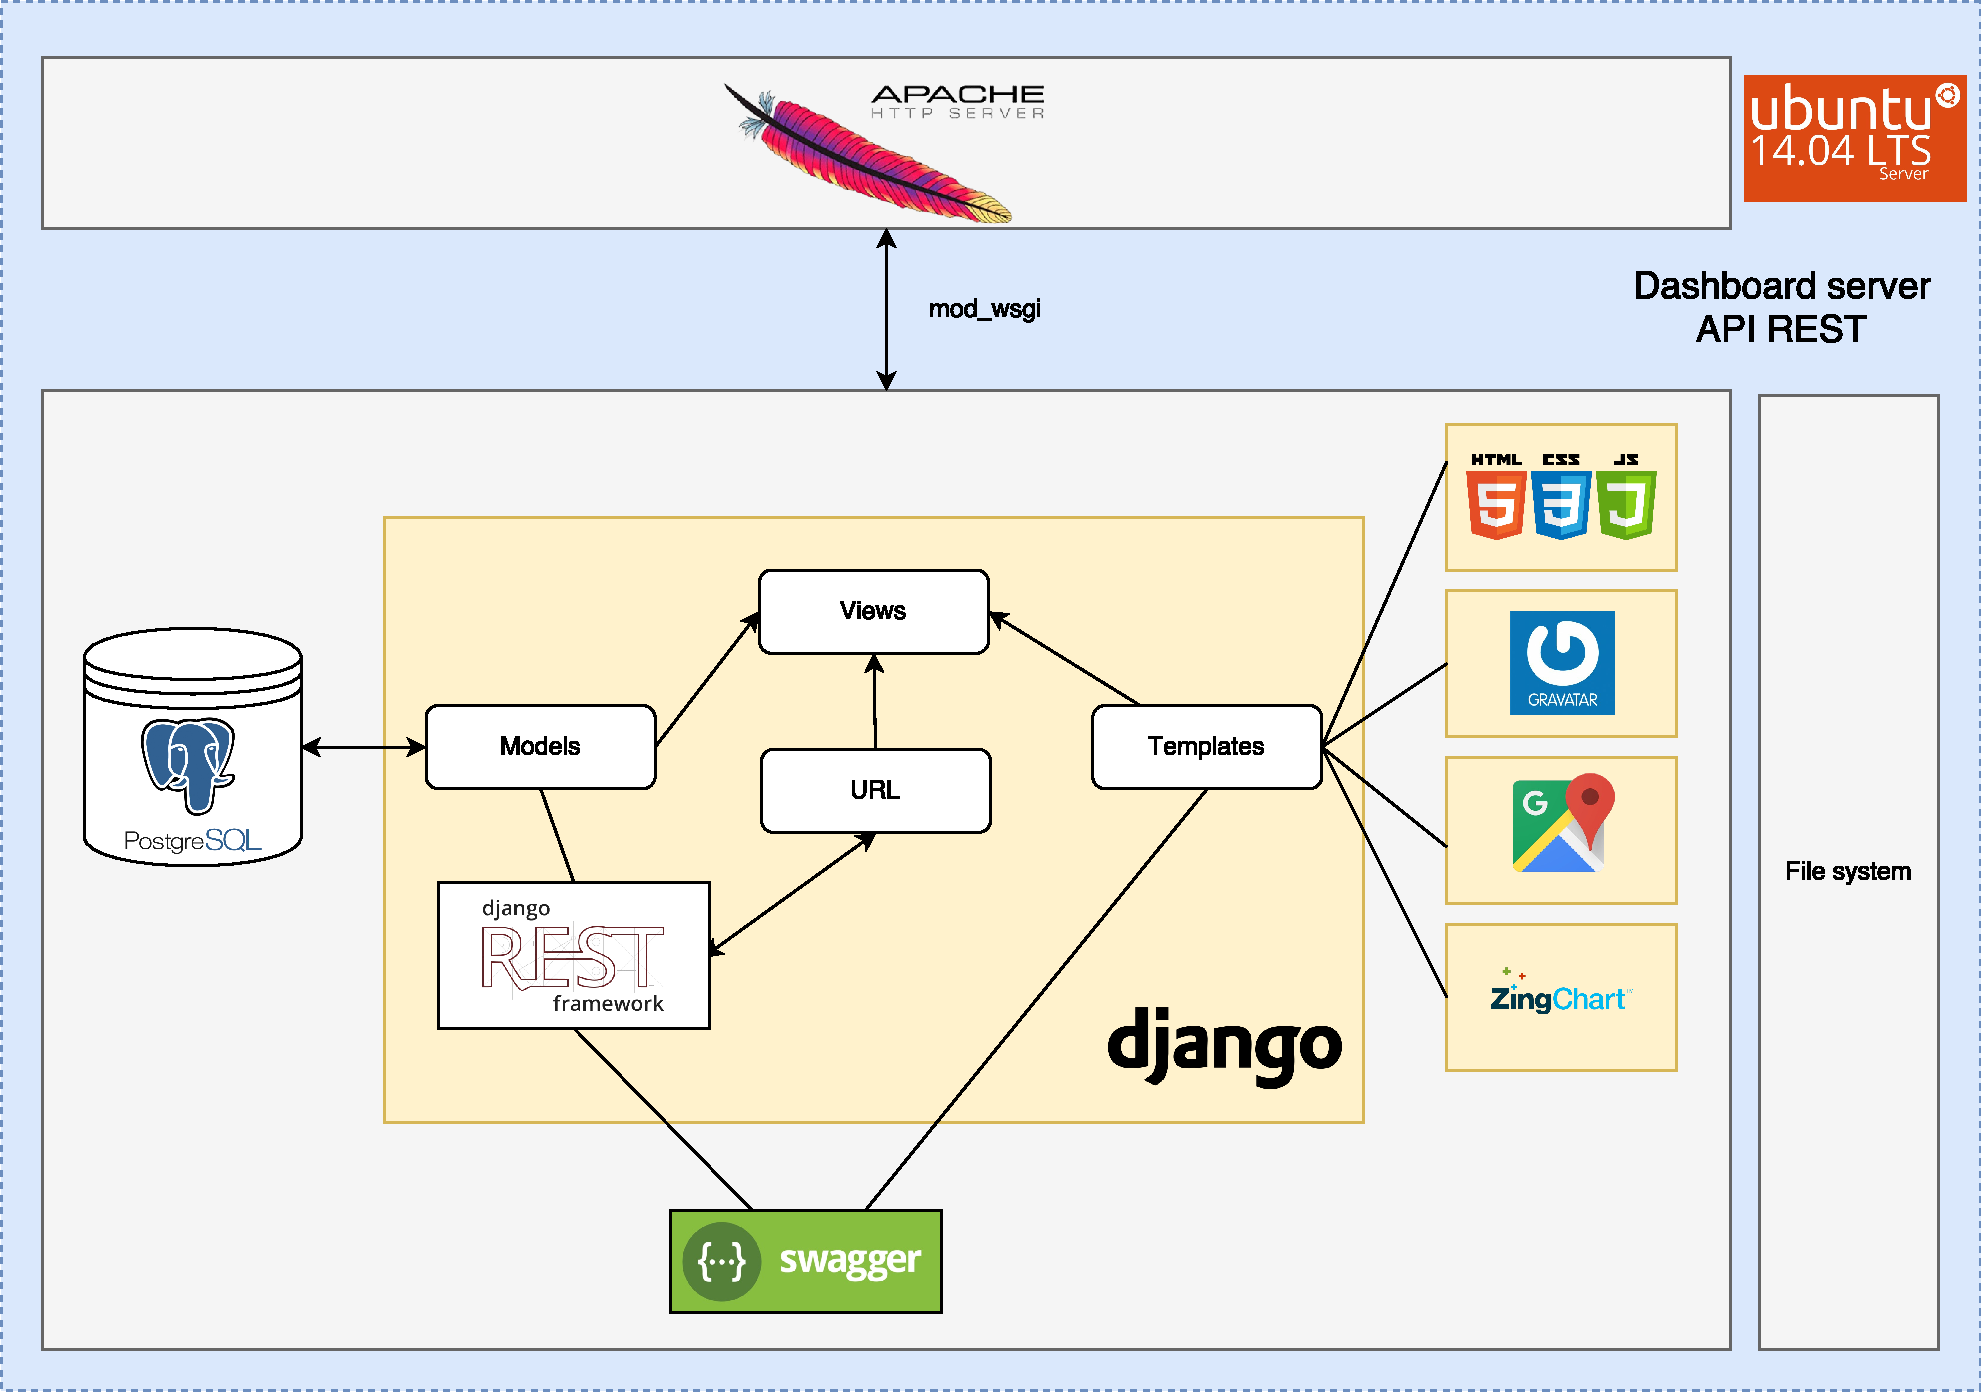
\includegraphics[width=\linewidth]{esquemas/fisica-si.pdf}
	\caption{Arquitetura do sistema de informação (\textit{dashboard}, base de dados e API)}
	\label{arquiteturasi}
\end{figure}



\subsubsection{Aplicação web}

A aplicação web é um componente essencial, enquadrando-se na camada de lógica de negócio como também na camada de apresentação, permitindo a interação por parte do utilizador (\textit{frontend}) como também no processamento lógico (\textit{backend}).   

Tal como vimos na secção do Estado de Arte, a tecnologia para o desenvolvimento web recaiu sobre a \textit{framework} Django, mais precisamente na versão 1.11 para python 2.7, sendo que como \ac{IDE} foi utilizada a verão 2016.3.3 do PyCharm. Dada a facilidade com que esta \textit{framework} tem em manipular views e templates, optou-se que ambas as componentes (\textit{frontend}/\textit{backend}) fossem desenvolvidas recorrendo ao Django. Para além disso, optou-se por criar uma API REST que permitisse a manipulação dos dados existentes na base de dados, sendo esta também desenvolvida paralelamente com a aplicação web. Seguidamente será explicada a sua arquitetura.   

Um dos pontos mais interessantes no Django é sem dúvida a existência de \ac{ORM}. Consiste numa técnica de desenvolvimento que permite modelar os dados através de classes em Python. Através dela, é possível gerar tabelas na base de dados e manipulá-las sem a necessidade de interagir diretamente com \ac{SQL} (embora também seja possível). A verificação dos valores lidos pelos sensores e possível geração de alarmes é averiguado por um \textit{trigger} desenvolvido em \ac{SQL}, no capitulo \ref{implementacao} será explicada a sua implementação.  


Relativamente à escolha do \ac{SGBD} recaiu sobre o PostgreSQL, mais concretamente na versão xxx. Como ferramenta gráfica para administração deste \ac{SGBD} foi utilizado o PgAdmin III\footnote{www.pgadmin.org/} na versão 1.22. Este software gráfico tem inúmeras funcionalidades desde a possibilidade de ligação a base de dados remotas até à adição, edição, remoção e  consultas em tabelas. Esta ferramenta é \textit{opensource} e encontra-se disponível para Windows e UNIX. Como vimos no capitulo \ref{state}, este \ac{SGBD} permite uma grande facilidade de incorporação a um projeto em Django. 


No que diz respeito à camada de apresentação na plataforma web foram utilizadas as seguintes bibliotecas/\textit{frameworks}: 

\begin{itemize}
	\item \textbf{\acs{HTML}, \acs{CSS} e \acs{JS}}: o ponto de partida para a criação da interface web assentou no template denominado por AdminLTE\footnote{https://adminlte.io/} sendo este baseado em Bootstrap 3\footnote{http://getbootstrap.com/}. Neste template prevalecem as seguintes características:  design responsivo, interface leve e apelativa, existência de múltiplos plugins, compatibilidade entre navegadores entre outros. 
	
	\item \textbf{Gravatar}: serviço que disponibiliza um avatar que esteja associado a endereços de email registado. O Gravatar disponibiliza uma API que pode ser utilizada nas mais diversas linguagens de programação\cite{gravatar}.
	 
	\item \textbf{\ac{API} Google Maps}: consiste num serviço de visualização de mapas e imagens de satélite, desenvolvido pela Google. É usado na visualização da localização dos módulos de sensores. 
	
	\item \textbf{ZingChart}: biblioteca em \ac{JS} que permite receber dados a apresentá-los em formato gráfico. Esta solução \textit{opensource} disponibiliza mais de 35 tipos e módulos de gráficos. 
\end{itemize}





\subsubsection{\acs{API} \acs{REST}}


Os métodos desta \ac{API} permitiram execuções funções do tipo \ac{REST}. A tecnologia \ac{REST} foi apresentada por Roy Fielding na Universidade de Califórnia no ano de 2000, cujo o titulo da sua dissertação era "Architectural Styles and the Design of Network-based Software Architectures". Roy estudou um conjunto de arquiteturas de software que usam a Web como uma plataforma para computação distribuída\cite{Rodriguez2015}. Esta tecnologia define um conjunto de princípios que possibilitam desenhar serviços web com base nos recursos do sistema, considerando a forma com os recursos são coordenados e transferidos através de \ac{HTTP} para vários clientes nas mais diversificadas linguagens. 

Os métodos da API permitem executar as funções \ac{REST} usando métodos \ac{HTTP} explicitamentee. Assim, torna-se fundamental perceber estes métodos para ter um melhor conhecimento do funcionamento da \ac{API}. Seguidamente são descritos os métodos mais importantes que dão suporte a cada uma das funções \ac{REST}.


\begin{itemize}
	\item \textbf{GET}: permite efectuar operações de leitura 
	\item \textbf{POST}: permite realizar operações de escrita, permitindo criar novos recursos ao sistema.
	\item \textbf{PUT}: permite criar ou atualizar um novo objecto ao sistema 
	\item \textbf{DELETE}: permite apagar objecto ou recurso ao sistema. 
\end{itemize}




Como vimos no capítulo \ref{state}, a escolha da \textit{framework} para construção desta \ac{API} \ac{REST} recaiu sobre o \textit{Django REST framework}. Esta framework possui uma extensa documentação e um elevado apoio da comunidade que a utiliza, sendo uma das mais utilizadas e incorporadas em projetos Django. 

Relativamente à autenticação desta \ac{API}, optou-se por utilizar um esquema de autenticação fundamentado no mecanismo de autenticação \ac{HTTP} baseado em \textit{tokens}\cite{tokenREST}. Neste mecanismo, o cliente primeiramente troca as suas credencias (username e password) por um token, seguidamente, em vez de enviar essas credenciais a cada requisição, o cliente apenas enviará o token inicialmente recebido, permitindo assim o acesso aos conteúdos pretendidos, com respetiva autenticação e autorização dos mesmos (figura \ref{autnetAPI}).


\begin{figure}[h]
	\centering
	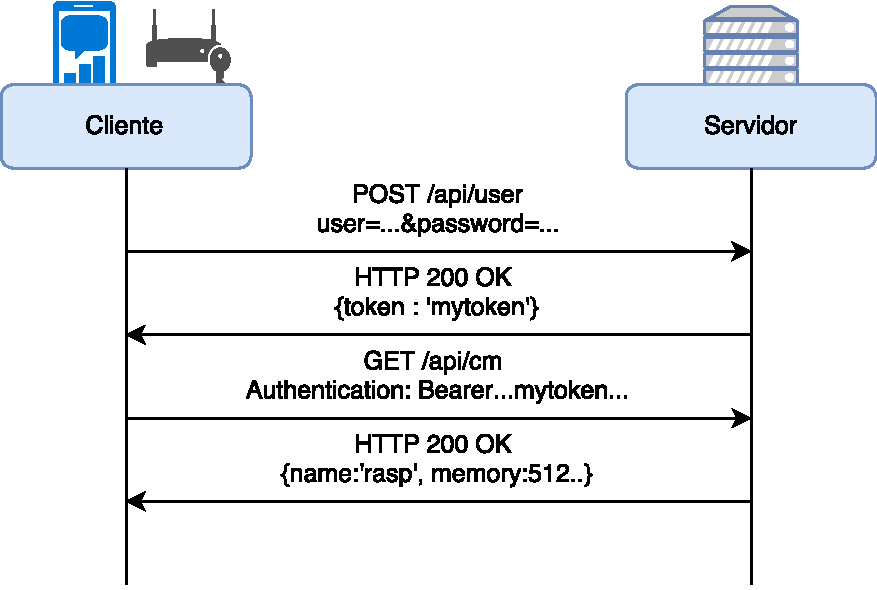
\includegraphics[scale=0.61]{esquemas/autenticacaohttpesquema.pdf}
	\caption{Processo de autenticação em HTTP através de token (adaptado de \cite{AdoKukic2016})}
	\label{autnetAPI}
\end{figure}


Resumidamente e com o objetivo de explicar o esquema da figura \ref{autnetAPI}, são enumerados os passos de autenticação em HTTP via token. 

\begin{enumerate}
	\item O cliente envia as credenciais para um servidor.
	\item O servidor valida e autentica essas credenciais gerando consequentemente um token.
	\item O servidor envia o token para o cliente.
	\item O cliente guarda o token e este é enviado sempre que existe uma requisição através do cabeçalho do protocolo HTTP. 
	\item O servidor, em cada requisição verifica se o token é válido ou não. Caso seja, o servidor aceita a requisição, caso contrário esta é rejeitada.
	\item O servidor pode ter um endpoint que renova o token sempre que necessário. 
\end{enumerate}




Na tabela \ref{endpointsapi} encontram-se todos os endpoints e respectivas funções (POST/GET/PUT) a implementar. Seguidamente será descrito como foi implementada a documentação desta API.  


\begin{table}[h]
	\centering

	\begin{tabular}{|l|l|l|l|l|}
		\hline
		\rowcolor[HTML]{C0C0C0} 
		\multicolumn{1}{|c|}{\cellcolor[HTML]{C0C0C0}\textbf{Endpoints da API REST}} & \multicolumn{1}{c|}{\cellcolor[HTML]{C0C0C0}\textbf{POST}} & \multicolumn{1}{c|}{\cellcolor[HTML]{C0C0C0}\textbf{GET}} & \multicolumn{1}{c|}{\cellcolor[HTML]{C0C0C0}\textbf{PUT}} & \multicolumn{1}{c|}{\cellcolor[HTML]{C0C0C0}\textbf{DELETE}} \\ \hline
		/api/user/ & \checkmark & \checkmark &  &  \\ \hline
		/api/user/\{pk\_or\_username\}/ &  & \checkmark & \checkmark & \checkmark \\ \hline
		/api/smpercm/ &  & \checkmark &  &  \\ \hline
		/api/smpercm/\{pk\_or\_name\_cm\} & \checkmark & \checkmark &  &  \\ \hline
		/api/sm/ & \checkmark & \checkmark &  &  \\ \hline
		/api/sm/\{pk\_or\_name\}/ &  & \checkmark & \checkmark & \checkmark \\ \hline
		/api/sensortype/ & \checkmark & \checkmark &  &  \\ \hline
		/api/sensortype/\{pk\_or\_name\} &  & \checkmark & \checkmark & \checkmark \\ \hline
		/api/sensorpersm/\{id\_sm\_or\_name\_sm\} & \checkmark & \checkmark &  &  \\ \hline
		/api/sensor/ &  & \checkmark &  &  \\ \hline
		/api/sensor/\{pk\_or\_sensor\_type\} & \checkmark & \checkmark &  &  \\ \hline
		/api/reading/\{id\_sensor\}/\{date\_start\}/\{date\_end\} & \checkmark & \checkmark &  &  \\ \hline
		/api/communication/\{pk\_or\_name\}/ &  & \checkmark & \checkmark & \checkmark \\ \hline
		/api/cm/ & \checkmark & \checkmark &  &  \\ \hline
		/api/cm/\{pk\_or\_name\}/ &  & \checkmark & \checkmark & \checkmark \\ \hline
		/api/alarmssettings/\{id\_sensor\} & \checkmark & \checkmark &  &  \\ \hline
		/api/alarms\_sensor/\{id\_sensor\} & \checkmark & \checkmark &  &  \\ \hline
		/api/alarms\_reading/\{id\_reading\} & \checkmark & \checkmark &  &  \\ \hline
	\end{tabular}
	\caption{Endpoints da API REST e respetivos métodos a implementar}
	\label{endpointsapi}
\end{table}






\subsubsection{Documentação interativa}


Para a geração automática da documentação da API utilizou-se o Swagger. Tal como descrito no site oficial desta framework\cite{SmartBearSoftware2017}, o Swagger é considerado a ferramenta de APIs mais popular e completa de todo o mundo permitindo facilmente o desenvolvimento do ciclo de vida de uma \ac{API}, desde o design, documentação, testes e também implementação, tendo a grande vantagem de ser \textit{opensource}. Neste contexto, apenas será utilizada como documentação, de modo a facilitar a interpretação da \ac{API} criada. O Swagger possui uma interface apelativa e intuitiva, permitindo interagir com a \ac{API} de modo que os seus utilizadores tenham uma ideia geral de como esta responde aos pedidos para diversos parâmetros e opções. 





\subsubsection{Implementação do sistema}

Para implementação do projeto anteriormente descrito e respetiva API, foi-me fornecida uma máquina com um distribuição Linux (Ubuntu 14.04.5) com as seguintes características: 

\begin{itemize}
	\item \ac{CPU}: Intel(R) Xeon(R) CPU E5-2670 v3 @ 2.30GHz
	\item \ac{RAM}: 2 GB
	\item Disco: 10.7 GB
\end{itemize}


Para o processo de \textit{deployment} deste projeto optou-se pela utilização do servidor Apache juntamente com o pacote mod\_wsgi\footnote{https://modwsgi.readthedocs.io/en/develop/}. 
Este pacote fornece uma \ac{WSGI} compatível para o alojamento de aplicações web em Python sob o servidor \ac{HTTP} Apache. O Apache é um servidor web \textit{opensource} mais utilizado em todo o mundo\cite{TheApacheSoftwareFoundation2016}.







% implementação falar da incorporação na dashboard e poss





%\section{Documentação automática}

%\subsection{Documentação API}












\subsubsection{Aplicação mobile}


Após a analise de requisitos da aplicação mobile, optou-se por elaborar um protótipo da aplicação mobile antes de proceder à sua real implementação. O \textit{mockup} da aplicação apresenta-se no Apêndice X. 

\begin{figure}[h]
	\centering
	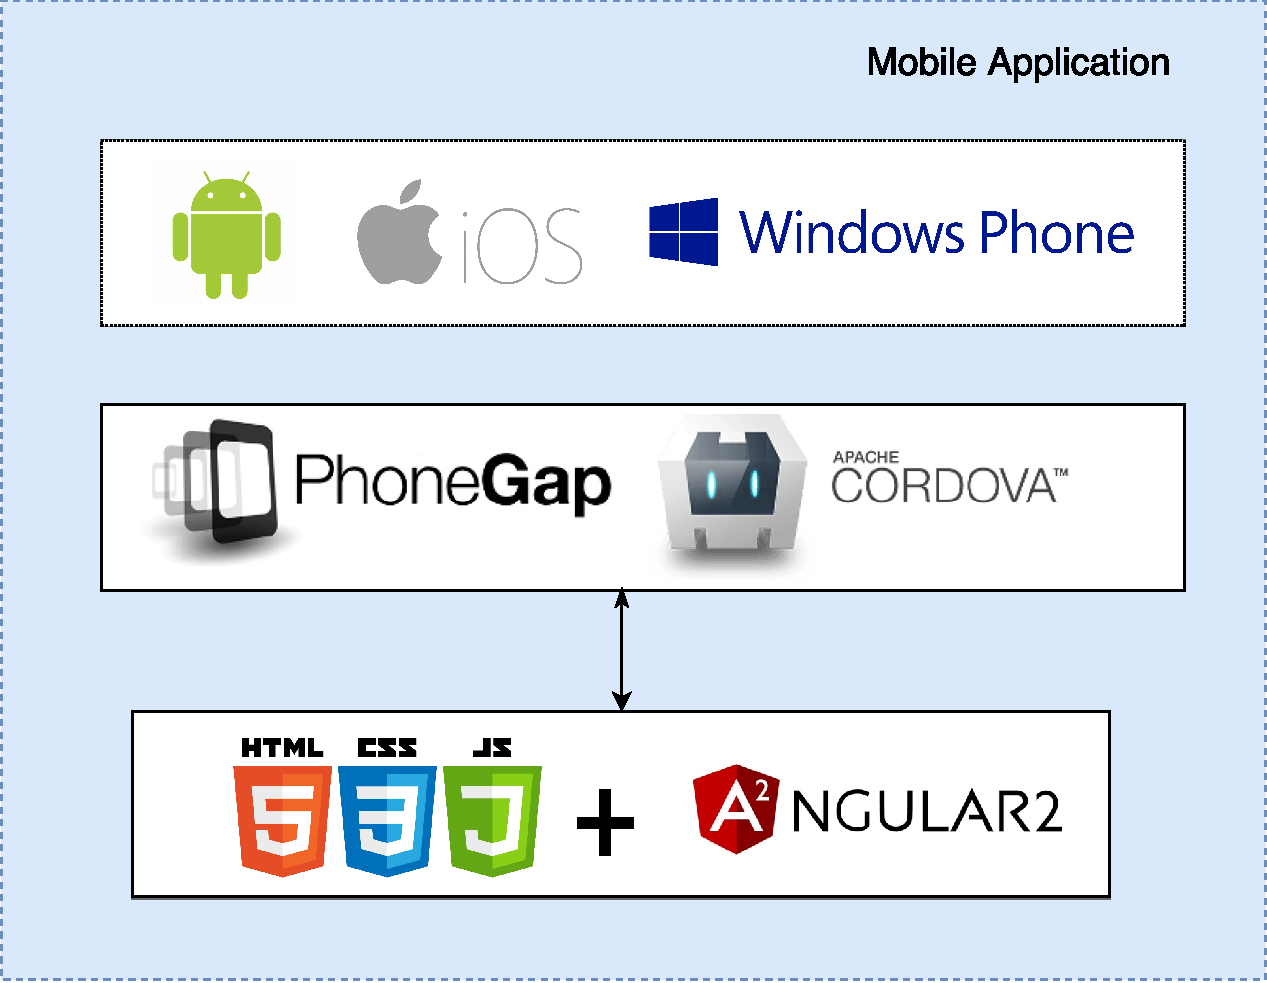
\includegraphics[scale = 0.5]{esquemas/arquitetura-mobile.pdf}
	\caption{Arquitetura da aplicação mobile}
	\label{arquiteturamobile}
\end{figure}


Tal como descrito no capitulo \ref{state}, para o desenvolvimento do aplicativo mobile optou-se pela utilização de um paradigma multi-plataforma, mais concretamente a \textit{framework} Phonegap. Esta framework utilizada a tecnologia Cordova da Apache que permite a integração com recursos nativos dos dispositivos. Através dela, é possivel desenvolver aplicações móveis utilizando simplesmente \ac{HTML}, \ac{CSS} e \ac{JS} sem a necessidade de depender de APIs específicas. De modo a facilitar a manipulação do \ac{JS} optou-se por utilizar a \textit{framework} AngularJS. Esta framework \textit{opensource} mantida pela google desde 20XX 



VAMOS USAR ANGULAR 2




Consumir a API REST 

Consumir a API REST 
Consumir a API REST 


\subsection{Simulação em \textit{hardware}}


Após a desenvolvimento da API, pretendeu-se simular o sistema num contexto real. Para tal, pretendeu-se encontrar hardware que encaixasse no contexto deste projeto. Foram utilizados dois micro-controladores (Arduino e Raspberry Pi 3) e alguns sensores. Para este cenário, assume-se que o Arduino é considerado um \acl{SM} que possui um conjunto de sensores enquanto que o Raspberry Pi 3 é um \acl{CM} que recebe os dados provenientes do \acl{SM} enviando-os para o servidor.  

Seguidamente, são apresentados os sensores utilizados bem como os tipos de comunicação. 
 
\newpage
\subsubsection{Sensores utilizados}

Nesta secção serão apresentados os sensores utilizados na simulação e as suas principais características. Todos os sensores foram escolhidos tendo em conta o seu enquadramento no projeto e a sua disponibilidade em laboratório, sendo que serão ligados ao Arduino Nano. \\


\textbf{Temperatura}


Como sensor de temperatura foi utilizado um termístor do tipo \ac{NTC}. Como vimos no capítulo \ref{state}, um termístor é um semicondutor sensível à temperatura, ou seja, quando o coeficiente de variação da resistência com a temperatura é negativa, então a temperatura sobe e consequentemente a resistência diminui. Na figura \ref{esquema-temp} encontra-se o esquema de ligação deste componente e na tabela \ref{table-temp} as suas propriedades principais. 


\begin{figure}[h]
	\centering
	\begin{minipage}[b]{0.4\textwidth}
		\centering
		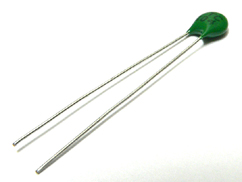
\includegraphics[width=\textwidth]{img/hardware/temperatura.jpg}
		\caption{Sensor TTC 104 NTC}
	\end{minipage}
	\hfill
	\begin{minipage}[b]{0.4\textwidth}
		\centering
		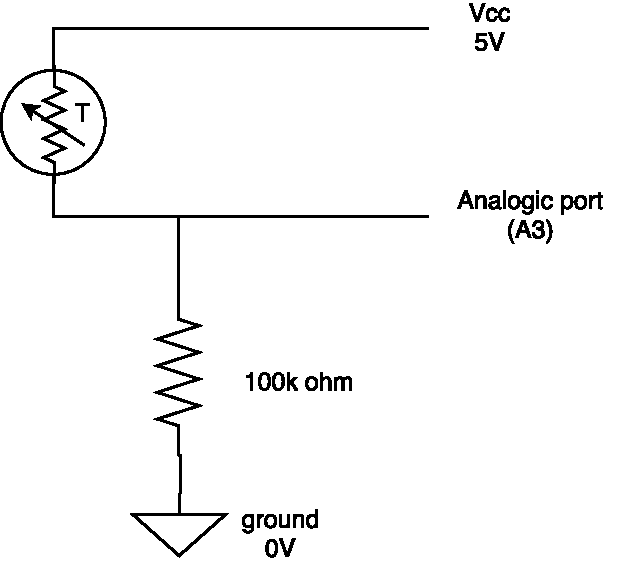
\includegraphics[width=\textwidth]{img/hardware/temp-esquema.pdf}
		\caption{Esquema eletrotécnico da ligação do sensor de temperatura}
		\label{esquema-temp}
	\end{minipage}
\end{figure}


\begin{table}[h]
	\centering
	
	\begin{tabular}{|
			>{\columncolor[HTML]{C0C0C0}}l |l|} \hline
		Dimensão & 5mm \\ \hline
		Resistência & 100 K$\Omega$  \\ \hline
		Valor máximo & +125 $^{\circ}$C \\ \hline
		Valor mínimo & -30 $^{\circ}$C \\ \hline
		Nível de confiança & + - 10\% \\ \hline
		Preço & 0.35 \euro/unidade \\ \hline
	\end{tabular}
	\caption[Características do sensor TTC 104]{Características do sensor TTC 104 \cite{temp-dta}}
	\label{table-temp}
\end{table}



\textbf{Luminosidade}

Para simular a luminosidade incidente foi utilizado um sensor do tipo foto-resistência. Este sensor, também conhecido como \ac{LDR}, não é mais do que uma resistência variável cujo o seu valor varia conforme a intensidade da luz que incide sobre ele, isto é, à medida que a intensidade da luz aumenta, a sua resistência diminui. Este sensor tem múltiplas aplicações, entre as quais se destaca a monitorização solar, indicador da posição do sol (up/down), alarmes anti-roubo, alarme para abertura/fecho de portas entre outras. Como vimos no capítulo \ref{state} é um sensor de baixo custo e bastante fácil de utilização. Na figura \ref{lum-esquema} encontra-se o esquema de ligação do componente e na tabela \ref{lum-cara} são apresentadas as principais características do sensor utilizado. 







\begin{figure}[h]
	\centering
	\begin{minipage}[b]{0.4\textwidth}
		\centering
		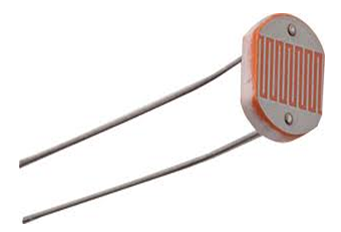
\includegraphics[width=\textwidth]{img/hardware/luminosidade.png}
		\caption{Sensor foto-resistência GL5528}
	\end{minipage}
	\hfill
	\begin{minipage}[b]{0.4\textwidth}
		\centering
		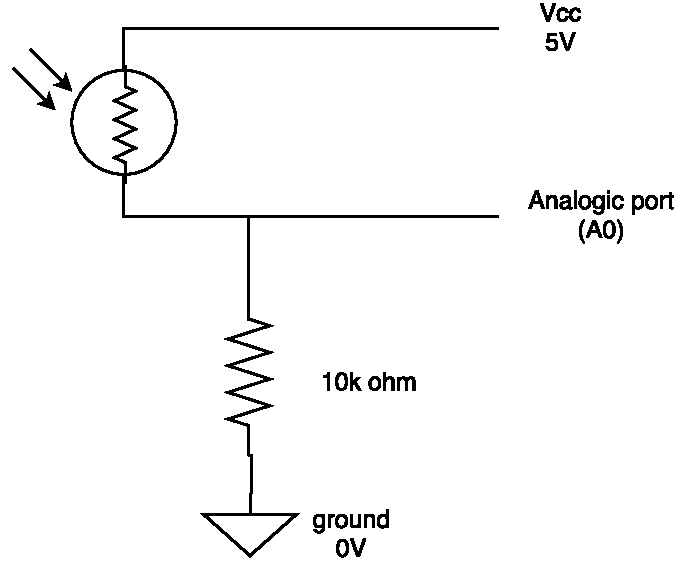
\includegraphics[width=\textwidth]{img/hardware/lumi_esquema.pdf}
		\caption{Esquema eletrotécnico da ligação do sensor de luminosidade}
		\label{lum-esquema}
	\end{minipage}
\end{figure}







\begin{table}[h]
	\centering
	
	\begin{tabular}{|
			>{\columncolor[HTML]{C0C0C0}}l |l|} \hline
		Diâmetro & 5mm \\ \hline
		Tensão máxima & 150VDC \\ \hline
		Potência máxima & 100mW \\ \hline
		Tensão de operação & -30 $^{\circ}$C a 70 $^{\circ}$C \\ \hline
		Espectro &540nm \\ \hline
		Comprimento com terminais & 32mm \\ \hline
		Resistência no escuro &1 M (Lux 0) \\ \hline
		Resistência na luz &10-20 Komega (Lux 10) \\ \hline
		Material & Carbono \\ \hline
		Preço & 0.22 \euro/unidade \\ \hline
	\end{tabular}
	\caption[Características do sensor GL5528]{Características do sensor GL5528 \cite{lum-data}}
	\label{lum-cara}
\end{table}




\textbf{Sensor para verificação do estado do nível de água}

Este sensor não é mais do que um interruptor que é ativo sempre que um determinado líquido ultrapassa o mesmo, isto é, sempre que algum líquido atingir o pedaço de plástico este irá subir ativando assim o circuito. Na figura \ref{esquem-liquido} encontra-se o esquema da ligação deste sensor.

\newpage


\begin{figure}[h]
	\centering
	\begin{minipage}[b]{0.4\textwidth}
		\centering
		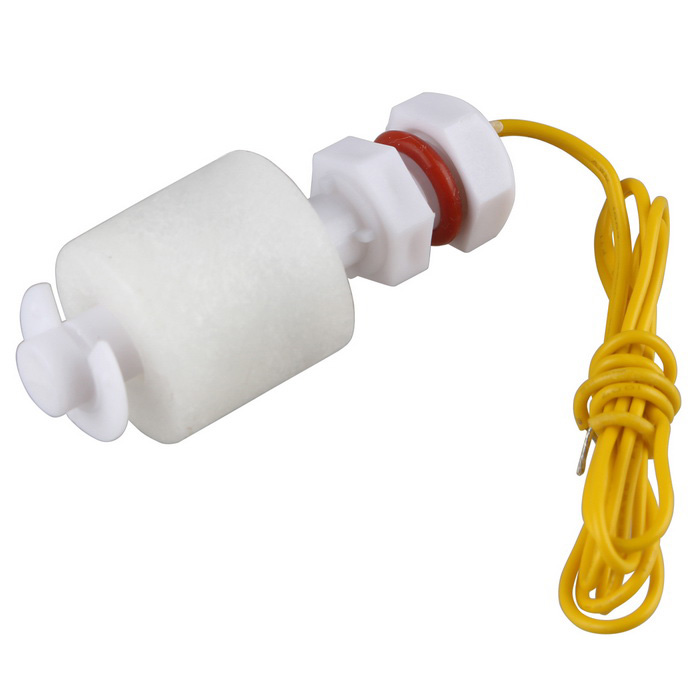
\includegraphics[width=\textwidth]{img/hardware/liquido.JPG}
		\caption{\textit{Water Level Switch Liquid Level Sensor Plastic Ball Float}}
	\end{minipage}
	\hfill
	\begin{minipage}[b]{0.4\textwidth}
		\centering
		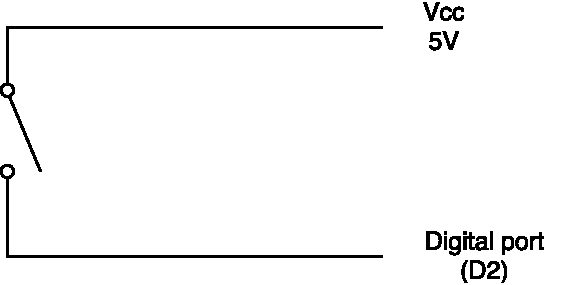
\includegraphics[width=\textwidth]{img/hardware/sw_esquema.pdf}
		\caption{Esquema eletrotécnico da ligação do sensor de nível líquido}
		\label{esquem-liquido}
	\end{minipage}
\end{figure}



\textbf{Simulador de válvula para transferências de águas}

Para a simulação de uma válvula que permitirá as transferência de água doce e/ou água salgada foi utilizado um \ac{LED}. Este possibilita facilmente identificar através da sua ativação se a válvula se encontra ativa ou não. 


\begin{figure}[h]
	\centering
	\begin{minipage}[b]{0.4\textwidth}
		\centering
		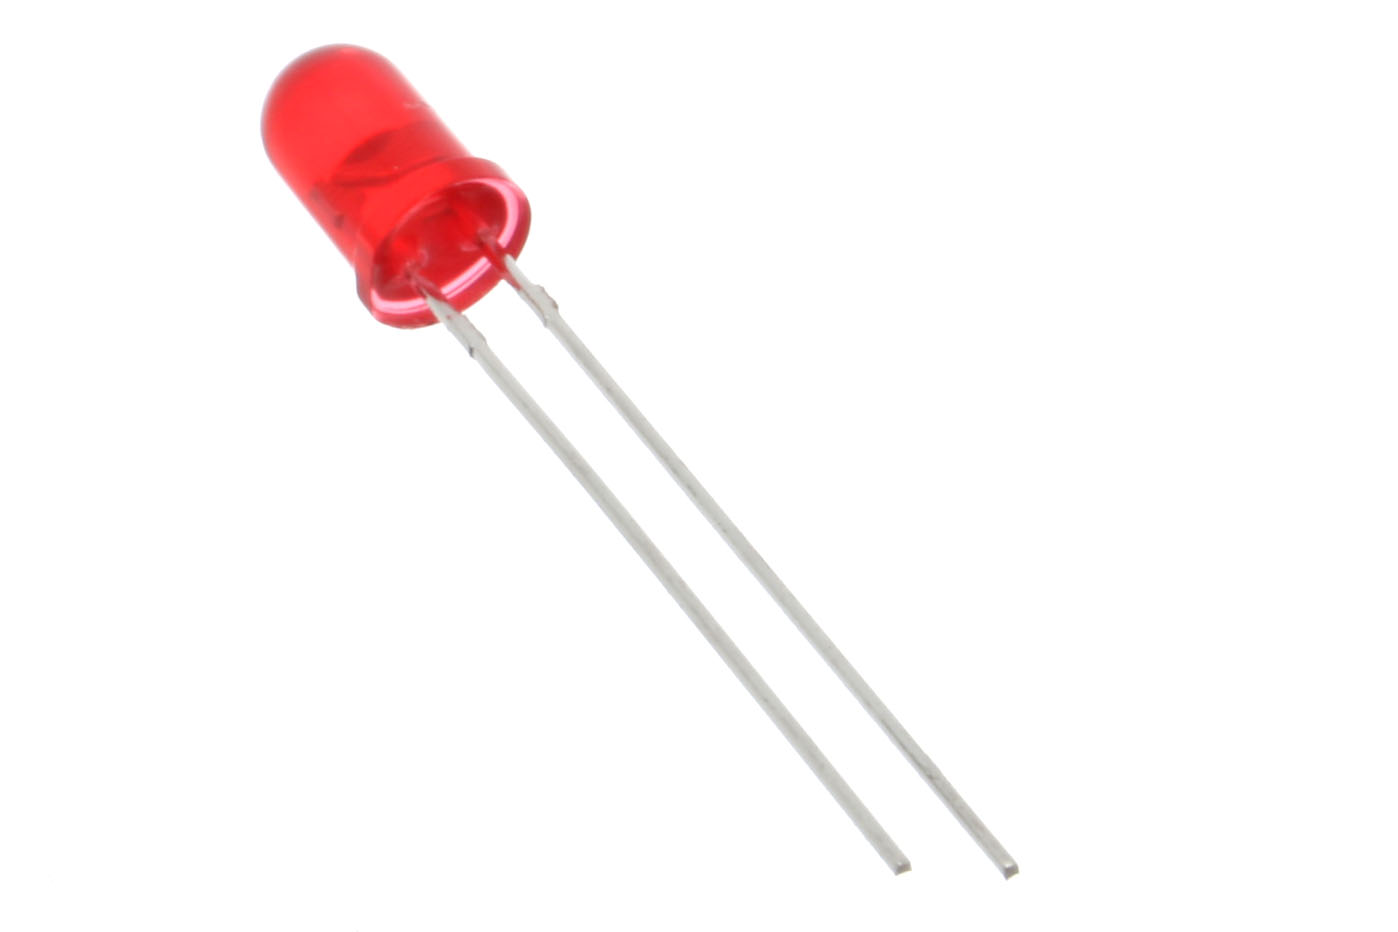
\includegraphics[width=\textwidth]{img/hardware/led.jpg}
		\caption{Led}
	\end{minipage}
	\hfill
	\begin{minipage}[b]{0.4\textwidth}
		\centering
		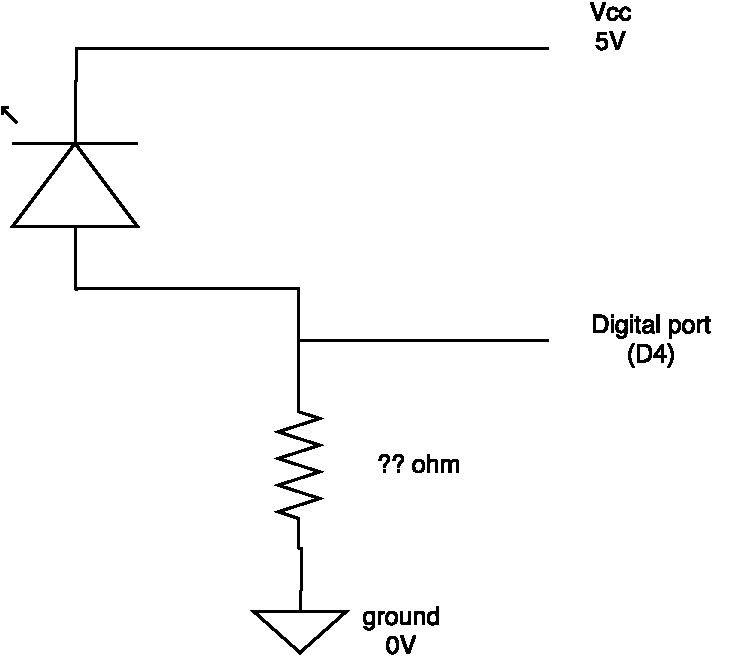
\includegraphics[width=\textwidth]{img/hardware/led_esquema.pdf}
		\caption{Esquema eletrotécnico da ligação do led}
	\end{minipage}
\end{figure}



\subsubsection{Comunicação}

Nesta secção, serão apresentados os tipos de comunicação para o cenário apresentado. Pretende-se que cada um dos módulo fique isolado entre si, o que implicou o estudo e respetiva escolha de algumas tecnologias de comunicações sem fio (secção XX do capítulo \ref{state}). Neste caso, foram escolhidas as seguintes: 

\begin{itemize}
	\item \textbf{Bluetooth}: utilizado para a comunicação entre o Arduino (\acl{SM}) e o Raspberry Pi 3 (\acl{CM}). No Arduino foi utilizado um módulo Bluetooth HC-06 e no Raspberry Pi 3 o seu próprio módulo interno. 
	\item \textbf{Wi-Fi}: utilizado para a comunicação entre o Raspberry Pi 3 (\acl{CM}) e o servidor web. 
\end{itemize}


O esquema da figura \ref{esquemcomm} pretende ilustrar os tipos de comunicação envolvidos nesta simulação para cada um dos componentes. 

\begin{figure}[!htb]
	\centering
	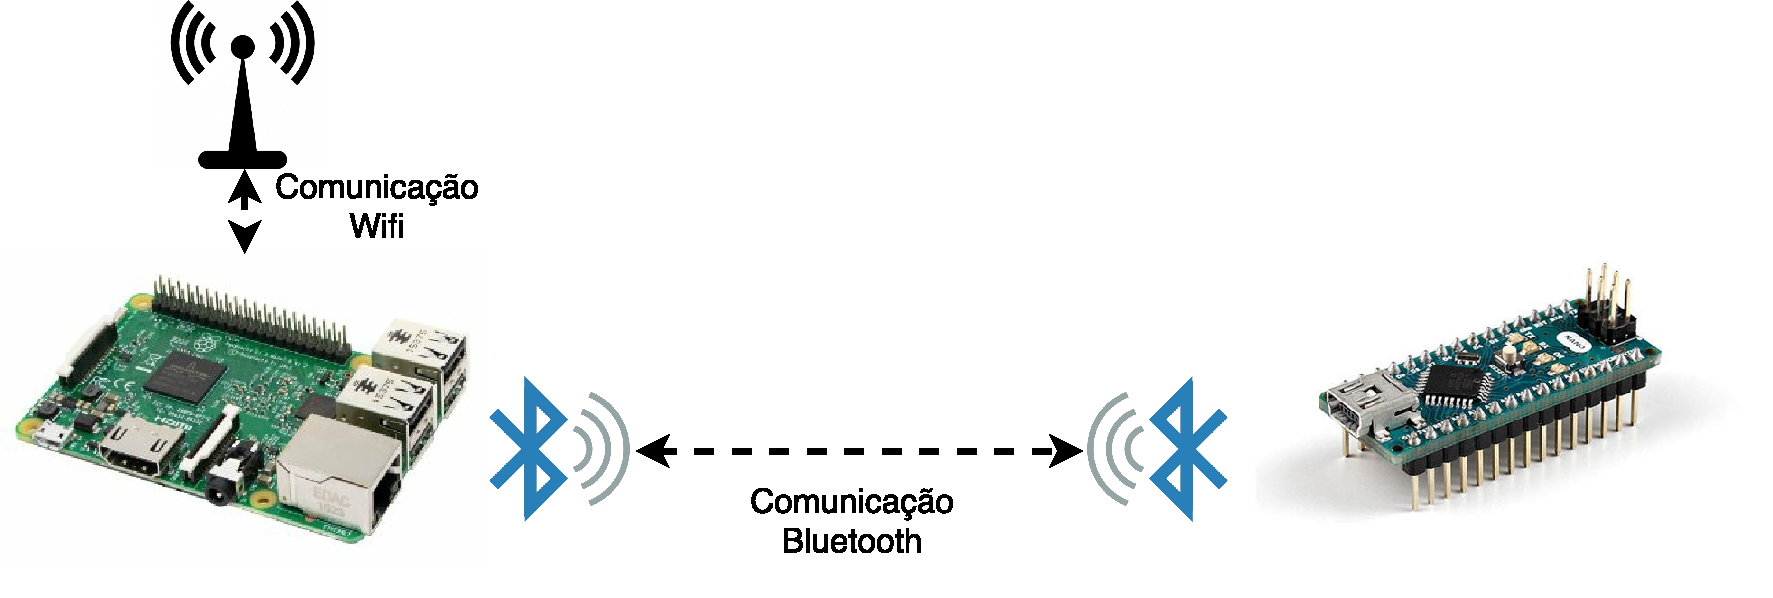
\includegraphics[width=\linewidth]{img/comm-blue/HW-geral.pdf}
	\caption{Comunicação entre componentes da simulação em hardware}
	\label{esquemcomm}
\end{figure}




\textbf{Módulo bluetooth HC-06}



Este módulo bluetooth oferece uma forma simples e barata de enviar e receber informações remotamente. Neste módulo existe um \ac{LED} que indica se este se encontra emparelhado com algum dispositivo. Na figura \ref{comimageesquema} encontra-se o esquema de ligação deste módulo e na tabela \ref{cara-comm} são apresentadas as suas principais características.



\begin{figure}[h]
	\centering
	\begin{minipage}[b]{0.4\textwidth}
		\centering
		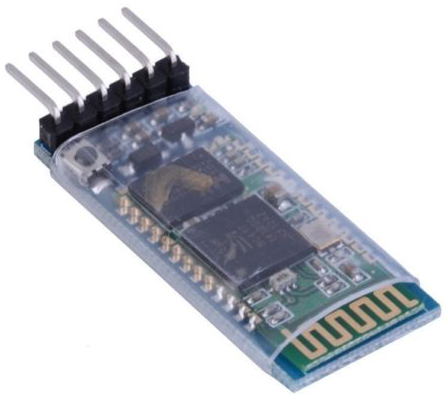
\includegraphics[width=0.7\textwidth]{img/hardware/bluetooth_zs-040.png}
		\caption{Módulo bluetooth HC-06}
		\label{comimage}
	\end{minipage}
	\hfill
	\begin{minipage}[b]{0.5\textwidth}
		\centering
		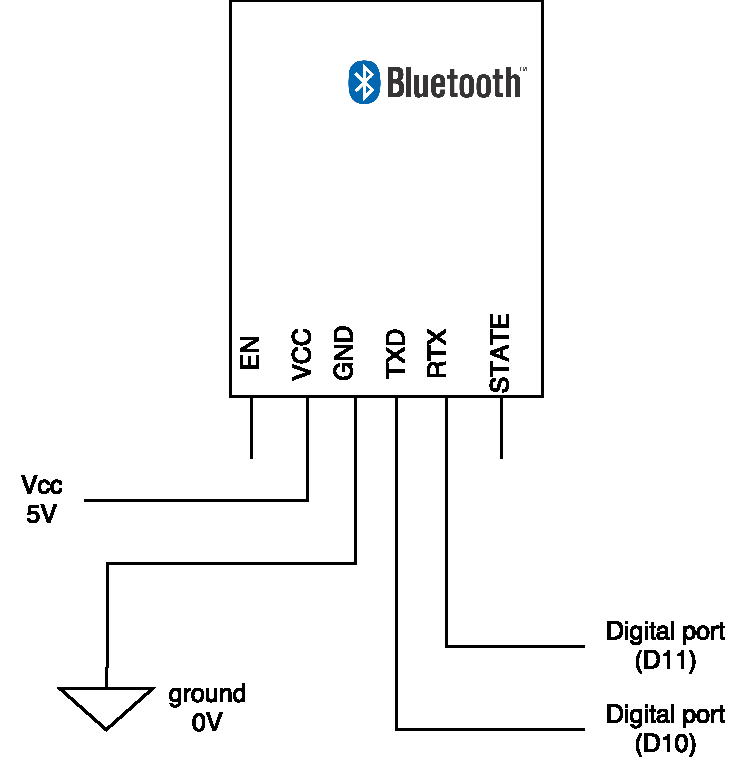
\includegraphics[width=0.6\textwidth]{img/comm-blue/electronic-sensors.pdf}
		\caption{Esquema eletrotécnico da ligação do módulo bluetooth}
		\label{comimageesquema}
	\end{minipage}
\end{figure}

\newpage

\begin{table}[h]
	\centering
	
	\begin{tabular}{|
			>{\columncolor[HTML]{C0C0C0}}l |l|} \hline		
		Versão bluetooth& v2.0 com \ac{EDR}\\ \hline 
		Frequência& 2,4GHz Banda \ac{ISM} \\ \hline
		Segurança& Autentificação (PIN) e Encriptação  \\ \hline
		Tensão& Aconselhada 3,3v (2,7v - 4.2v) \\ \hline
		Alcance& 10 metros \\ \hline
		Dimensões& 26,9 x 13 x 2,2mm \\ \hline
		Peso& 9,6g \\ \hline
		Temperatura (funcionamento)& -25C +75C \\ \hline 
		
		Preço&5.26 \euro /unidade  \\ \hline
	\end{tabular}
	\caption[Características do módulo bluetooth HC-06]{Características do módulo bluetooth HC-06 \cite{GuangzhouHCInformationTechnologyCo.2011}}
	\label{cara-comm}
\end{table}




%http://www.instructables.com/id/Modifying-the-AT-Codes-on-a-HC-05-With-the-Code-ZS/


%http://www.arduinoecia.com.br/2013/03/modulo-bluetooth-jy-mcu-configuracao.html







\section{Sistema de deteção de intrusos}


No contexto desta dissertação houve necessidade de implementar um sistema de video-stream que permitisse detetar intrusos, maioritariamente pessoas ou animais de grande porte, que possam invadir as quintas onde se produz Salicórnia. Esta necessidade prende-se essencialmente com elevado custo do \textit{hardware} do sistema de monitorização e também de eventuais instrumentos de elevado custo necessários ao cultivo desta espécie, como por exemplo,  geradores, máquinas elétricas para poda, entre outros.

Neste secção é descrita a tecnologia de processamento de imagem utilizada tal como o material necessário e respetiva arquitetura. 


\subsection{Biblioteca para processamento de imagem: OpenCV}

O OpenCV, também conhecido por \textit{Open Source Computer Vision Library}, é uma biblioteca de \textit{software} de visão por computador de código \textit{open-source} (figura \ref{opencvlogo}). 

\begin{figure}[!htb]
	\centering
	
\includegraphics[width=0.3\linewidth]{img/vision/opencv_logo.jpg}
	\caption{Logótipo OpenCV}
	\label{opencvlogo}
\end{figure}

Esta biblioteca possui mais de 2500 algoritmos otimizados, que inclui um conjunto abrangente de algoritmos clássicos e avançados de visão computacional bem como algoritmos de \textit{machine learning}. Esses algoritmos podem ser utilizados para os mais diversos fins, como por exemplo, para detectar e reconhecer rostos, identificar objetos, classificar ações humanas em vídeos, detetar movimentos numa câmara, seguir um objetos em movimento, produzir nuvens de pontos 3D de câmaras estéreo, entre outros. Esta biblioteca é amplamente utilizada em empresas e grupos de investigação, tendo interfaces nas mais diversas linguagens: C++, C, Python, Java e MATLAB, embora seja nativamente escrita na linguagem C. OpenCV tem mais de 47 mil pessoas na sua comunidade e excede os 7 milhões de downloads, tendo suporto para Windows, Linux e Mac OS\cite{Itseez}.




Desde logo, a escolha da tecnologia para processamento de imagem recaiu sobre o OpenCV não apenas por ser uma biblioteca bastante popular e possuir bastantes algoritmos implementados mas também por eu próprio possuir já algum \textit{background} e projetos desenvolvidos nesta área.  Pretendeu-se que este processamento fosse implementado em material já adquirido sem necessidade de gastos. Optou-se então por utilizar um \textit{Raspberry Pi 3} que juntamente com um \textit{Raspberry Pi camera module} (figura \ref{raspicam}) permitirá a aquisição de imagem e servirá também como \acl{CM} ao sistema de aquisição de dados. Na tabela \ref{cara-cam} apresentam-se algumas características deste módulo para o Raspberry Pi 3. 


\begin{figure}[!htb]
	\centering
	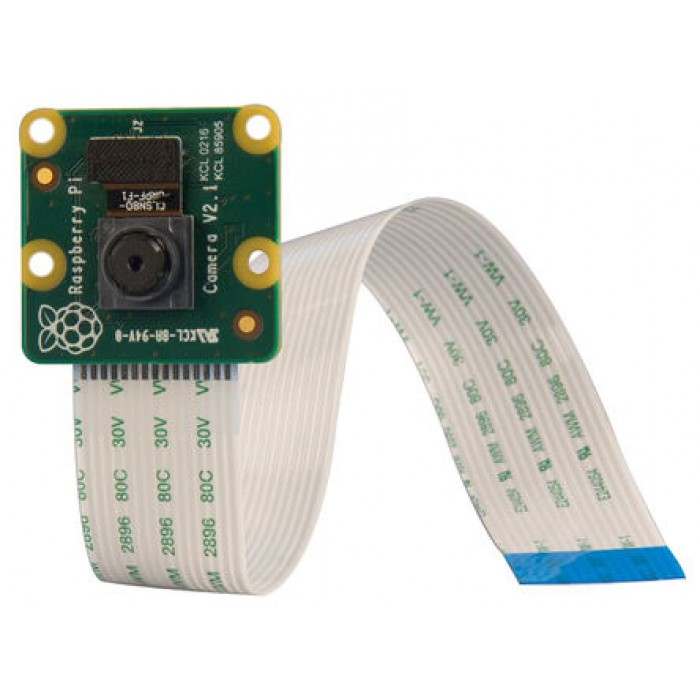
\includegraphics[width=0.3\linewidth]{img/hardware/camera_v2.jpg}
	\caption{Raspberry Pi Camera Board V2 8MP 1080p}
	\label{raspicam}
\end{figure}




\begin{table}[h]
	\centering
	
	\begin{tabular}{|
			>{\columncolor[HTML]{C0C0C0}}l |l|} \hline		
		Sensor & 8 megapixels Sony IMX219 \\ \hline
		Resolução de exibição & 1080p, 720p e 640x480p para vídeo \\ \hline
		Ligação à placa& Cabo fita curta (branca) \\ \hline
		Dimensões& 25 x 23 x 9 mm \\ \hline
		Peso& aproximadamente 3 g \\ \hline
		Compatibilidades& ultima versão do Raspbian \\ \hline
		Preço& 26,67 \euro /unidade  \\ \hline
	\end{tabular}
	\caption[Características do módulo bluetooth HC-06]{Características do Raspberry Pi camera module}
	\label{cara-cam}
\end{table}








Inicialmente, pretendeu-se explorar um algoritmo disponibilizado pelo OpenCV para a deteção de pessoas (corpo inteiro). Este algoritmo, juntamente com técnicas de \textit{machine learning}  permitem a deteção de pessoas numa determinada imagem e/ou vídeo. O \textit{machine learning} (em português aprendizagem automática) consiste num  método de análise de dados que automatiza o desenvolvimento de modelos analíticos, sendo usados algoritmos que aprendem interativamente a partir de dados recolhidos à priori\cite{Kotsiantis2007}. 

Após a realização de vários testes a este algoritmo, pretendeu-se implementar um servidor de \textit{streaming} que possa ser incorporado na \textit{dashboard}. Para tal, optou-se por criar um aplicação em Flask (\textit{framework} abordada no capitulo \ref{state}) que permita a aquisição de vídeo proveniente da  \textit{Raspberry Pi camera module} e realização do respetivo processamento. Esta aplicação web foi implementada num \textit{Raspberry Pi 3} tendo sido necessário optar por um servidor web, neste caso o NGINX\footnote{https://www.nginx.com/resources/wiki/}. O NGINX é um servidor HTTP de alto desempenho e open-source. É conhecido pela sua alta performance, estabilidade, configuração simples e baixo consumo de recursos\cite{Nginx2017}. 

Para comunicação entre o servidor web com a aplicação em Flask foi necessária a utilização de uma \ac{CGI} que permita gerir páginas dinâmicas, possibilitando ao navegador passar parâmetros para uma aplicação existente num servidor web. Optou-se por utilizar o uWSGI \footnote{https://uwsgi-docs.readthedocs.io}, sendo um dos mais populares. Na figura \ref{arquiteturavisao} encontra-se a arquitetura do sistema de deteção de intrusos e as respetivas tecnologias utilizadas.



\begin{figure}[h]
	\centering
	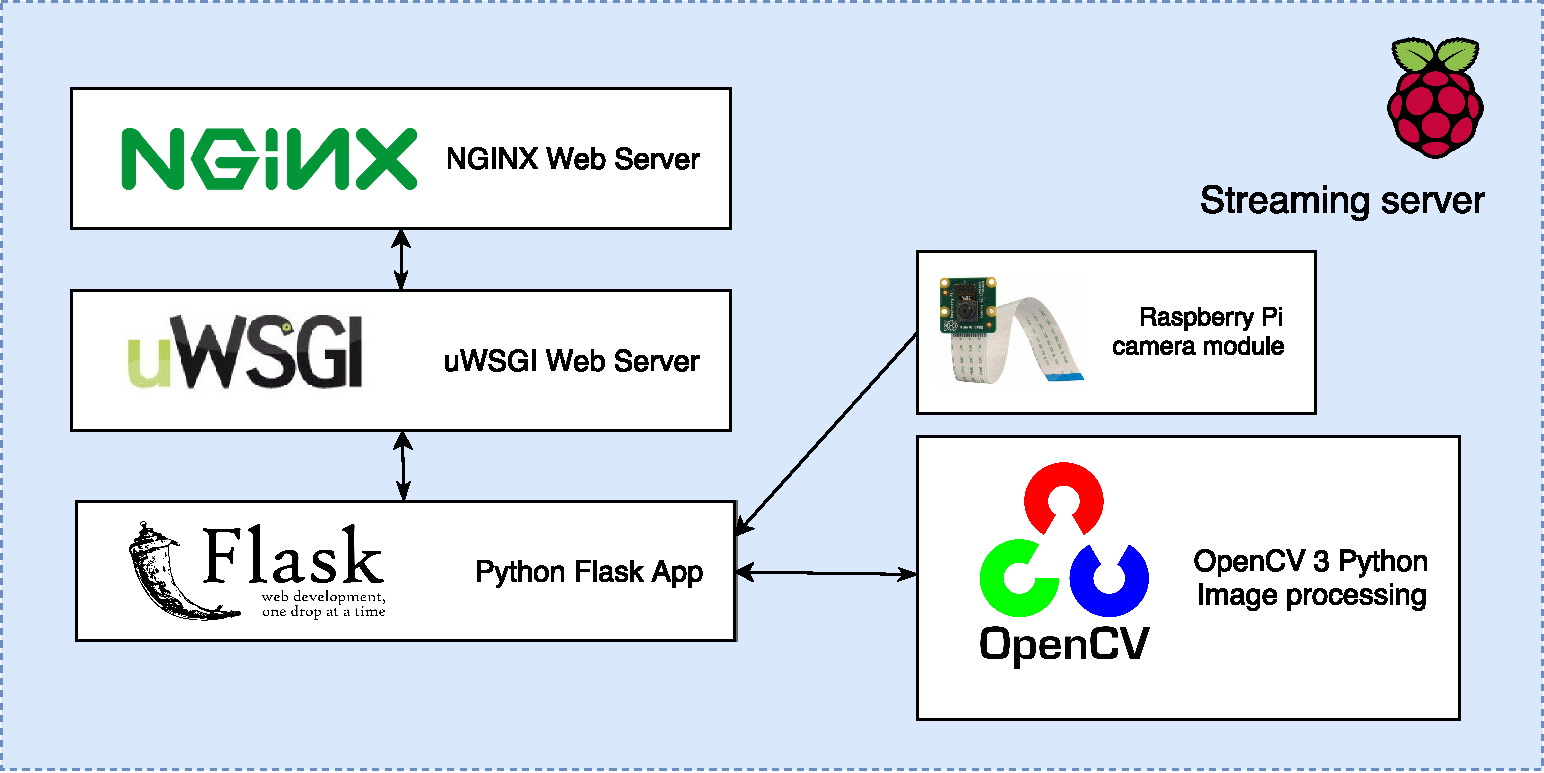
\includegraphics[scale = 0.5]{esquemas/videostream.pdf}
	\caption{Arquitetura do sistema de video stream}
	\label{arquiteturavisao}
\end{figure}




%%%%%%%%%%%%%%%%%%%%%%%%%%%%%%%%%%%%%%%%%%%%%%%%%%%%%%%%%%

\newpage
\section{Diagrama de componentes}

\begin{figure}[!htb]
	\centering
	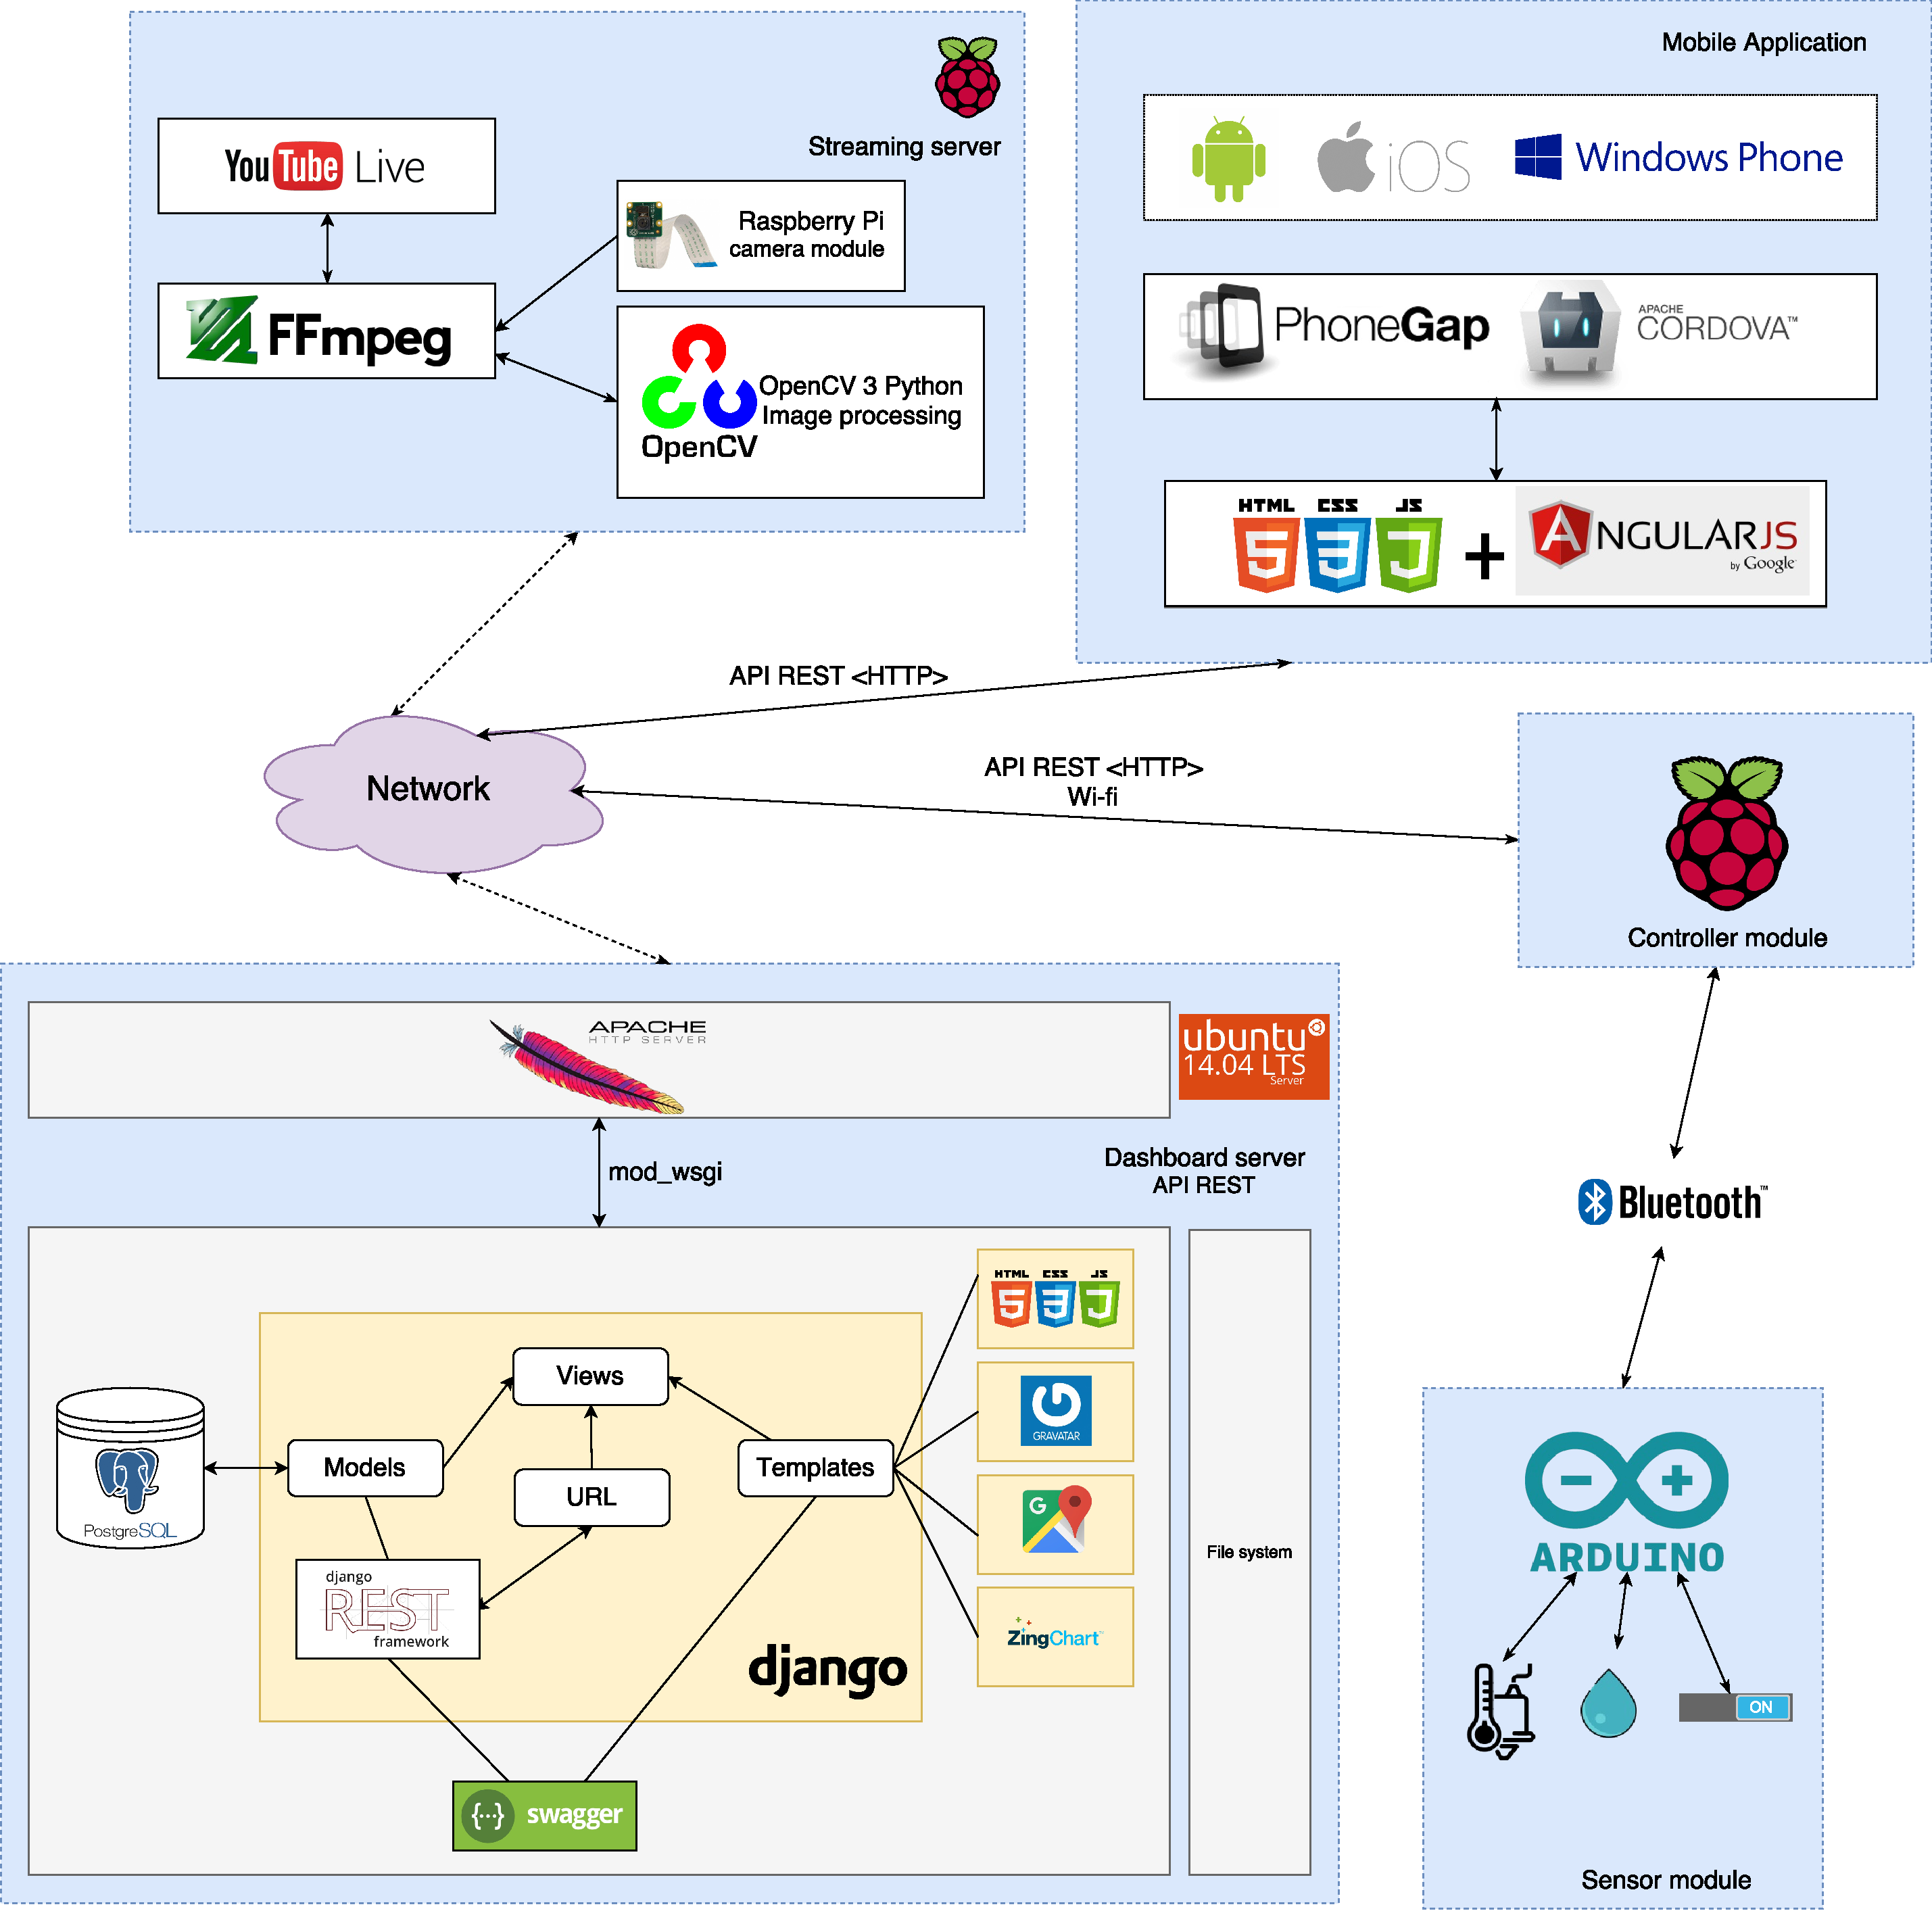
\includegraphics[width=\linewidth]{esquemas/arquitetura-final.pdf}
	\caption{Esquema relacional da estrutura da base de dados}
	\label{componentesall}
\end{figure}








\newpage








\section{Considerações finais}